\documentclass[]{tongjithesis}
\addbibresource[location=local]{tongjithesis.bib}
\usepackage[backend=biber,style=gb7714-2015]{biblatex}
\usepackage{lipsum}
\usepackage{duckuments}
\usepackage{color}
\usepackage{amsmath}
\numberwithin{equation}{chapter}
\usepackage{comment}
\usepackage{optidef}
\usepackage{tikz} % Import the tikz package
\usetikzlibrary{automata} % Import library for drawing automata
\usetikzlibrary{positioning} % ...positioning nodes
\usetikzlibrary{arrows} % ...customizing arrows
\tikzset{node distance=2.5cm, % Minimum distance between two nodes. Change if necessary.
		every state/.style={ % Sets the properties for each state
		semithick,
		fill=gray!10},
		initial text={}, % No label on start arrow
		double distance=2pt, % Adjust appearance of accept states
		every edge/.style={ % Sets the properties for each transition
		draw,->,>=stealth', % Makes edges directed with bold arrowheads
		auto,semithick}}
\let\epsilon\varepsilon

\school
{交通运输工程学院}
{School of Electronic and Information Engineering}

\major
{综合交通信息管理与控制}
{Automation}

\thesistitle
{共享单车调度模型研究与影响因素分析}
{}
{The Research on Multispectral Pedestrian Detection Based on the Visible and Infrared Image Fusion }
{}

\thesisauthor{李炘玲}{Xinling Li}

\schoolnumber{1753298}

\keyword
{共享单车,调度问题,网络流量模型}
{(Dockless) Bike-sharing, Fleet Relocation, Network Flow Model}

\advisor{沈煜}{Yu Shen}

\thesisdate{2021}{6}{1}

%\maketitle

\begin{document}

\begin{cabstract}
	为了提高共享单车网络的运行效率,共享单车调度被广泛应用于共享单车网络中,用于从将单车从过饱和的区域中运送到欠饱和区域中以实现不同区域的单车量平衡。本文首先对共享单车需求预测的方法进行了讨论,接着提出了一个网络流量模型用于解决单车调度的最优化问题,并通过处理新加坡义顺区的实际共享单车使用数据作为模型输入,验证了次模型的合理性和有效性。在此基础上,继续利用此模型对调度成本、调度用车数量、共享单车数量进行了对于网络最终收益的敏感性分析,分析结果显示系统收益与这些影响因素间有明显联系。本文中所讨论的方法为共享单车网络中的单车投放数量以及定价提供了参考,并给出了有关共享单车网络管理的一些建议。
\end{cabstract}

\begin{eabstract}
	To enhance the service quality of bikesharing programs, bike fleet relocation is widely applied to redistribute bikes from bike sufficient areas to bike shortage areas thereby making a better bike-rider balance across different areas. In this study, a network flow model is proposed to solve the optimal relocation problem of shared bikes, and is implemented with the actual dockless shared bike usage data from Yishun, Singapore, to demonstrate its effectiveness. A series of sensitivity analyses are performed to test the impact of the relocation cost, the number of bikes and truck trikes, and the usage price on bike relocation. The results reveal an apparent connection between the profitability of the system and the analyzed factors. This work offers a modeling framework to start and operate a bikesharing service by determining the number of bikes and trikes as well as price schemes. Some bikesharing regulation policies are also suggested.
\end{eabstract}

% toc
\toc

% main contents
\mainmatter

\chapter{绪~论}
\section{研究背景}
为了减少尾气排放,并解决城市出行第一和最后一公里的问题,过去的十几年里,共享单车的应用在全世界内快速增长。共享单车网络的发展过程可以分为三个阶段:
\begin{enumerate}
	\item 无锁免费共享单车
	\item 有桩基于押金的共享单车
	\item 基于信息系统的无桩共享单车\cite{demaio2009bike,shaheen2010bikesharing,fishman2016bikeshare}。
\end{enumerate}
第一、第二代共享单车系统通常被看作最基础的系统,他们缺乏有效的信息记录和管理设备,无法有效的进行单车管理和防止单车盗窃,所以最终大多走向失败。在第三代共享单车系统中,停车桩和自动缴费使得共享单车更加易于管理,而信息设备也使单车的追踪成为可能。伴随着科技的发展,这些设备同样也在不断的升级换代,从而提供了越来越优质的服务。近年来,随着移动信息服务的发展,新一代的共享单车系统——无桩共享单车系统逐渐占领了共享单车市场。这种系统中的车辆配备了移动支付模块,GPS芯片,成为了目前共享单车系统的主流运营模式。

无桩共享单车系统能够追踪系统中所有车辆的位置和状态,从而使得车辆的管理和维护更具实时性和有效性。然而,在现实中,无桩共享单车项目还是常常难以长期运营,最终走向破产。在中国,自2017年以来,带有GPS的共享单车项目发展尤其迅猛,各运营商对市场的竞争十分激烈。2017年,摩拜和ofo进入中国市场,并开始了激烈的市场竞争,大量投放共享单车。到2018年,这两个运营商共同占有了90\%的市场份额。但是到2019年初期,大多数共享单车运营公司都已经倒闭或面临倒闭的危机。这些项目的失败说明,在不同运营商都投放了大量共享单车到市场中时,为了更好的管理,运营商需要对共享单车的运营模式和规律有更深的理解。共享单车的过度投放会带来诸多问题,例如造成公共空间资源的浪费(如下图\ref{waste1}、\ref{waste2}所示),且并不能保证高利用率,但是投放不足又会减少运营商在市场中的份额和盈利能力,最终也会导致破产。
\begin{figure}[H]
	\centering
	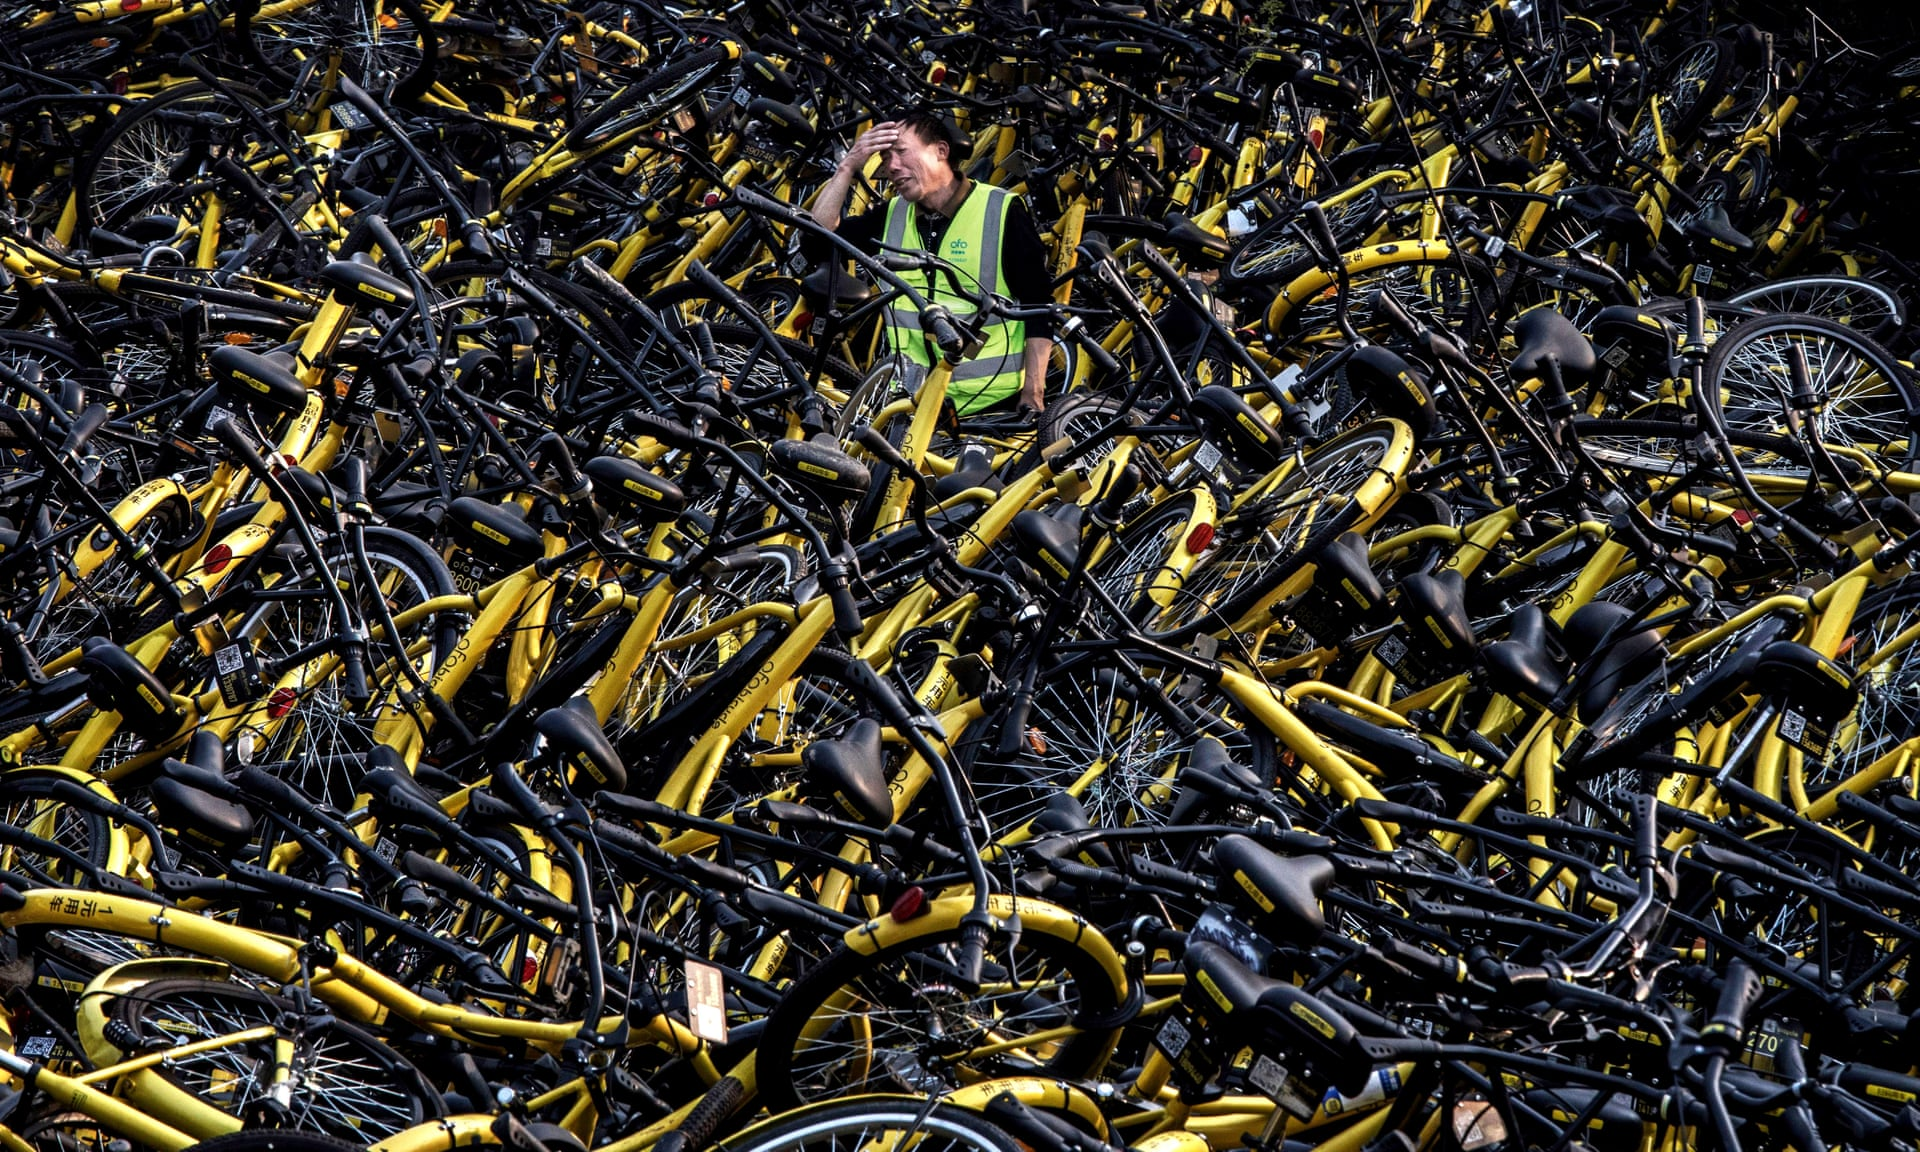
\includegraphics[width= 0.7 \textwidth]{figures_main/waste.jpg}
	\caption{共享单车过度投放(图片来源于网络)}
	\label{waste1}
\end{figure}

\begin{figure}[H]
	\centering
	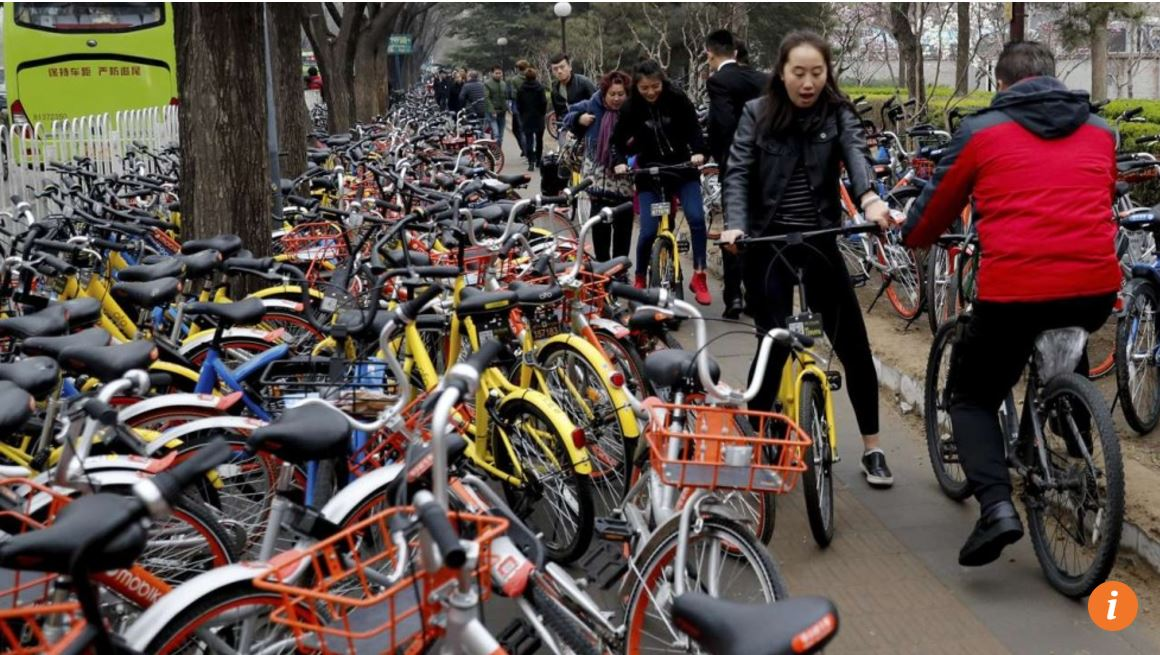
\includegraphics[width= 0.7 \textwidth]{figures_main/waste1.jpg}
	\caption{共享单车过度投放(图片来源于网络)}
	\label{waste2}
\end{figure}

平衡单车数量和盈利空间的方式之一就是使用调度。相比于购买更多的单车而言,调度更加可以更加灵活的调整共享单车系统提供服务的能力,可以在单车量适当的情况下,最大化运营商的盈利空间,所以也在共享单车的运营过程中被广泛使用。然而,调度计划的制订也需要进行仔细的考虑,因为共享单车系统通常分布面积广,过多的无效调度会给系统带来更高的运营成本,同样可能导致项目的破产。在这种背景下,对调度计划制订的讨论就显得尤为重要。在下一节中,我们将首先通过从新加坡最大的共享单车运营商之一的Obike公司获得的真实数据,讨论单车过度投放的问题,作为调度模型构建的基础。

\section{新加坡的无桩共享单车}
无桩共享单车在2017年第一次进入新加坡的共享单车市场,Obike就是最早开始的一批项目之一。在Obike的共享单车系统中,所有单车都配备了GPS定位仪,定位仪记录的数据使得对共享单车时空轨迹的刻画,以及对单车分布的分析成为了可能。本文的所有分析都是基于从Obike公司获取的2017年9月30日至11月1日的订单数据,每条订单数据中都包含起终点的位置以及时间信息。

通过对2017年10月17日一天的订单数据统计,得到共享单车的日分布如图\ref{spatial_aday}所示。图中的颜色越深,表示单车分布的数量越多。除了单车分布之外,下图中还显示了新加坡地铁站的位置和地铁线路的走向。从图中可以看出,共享单车在地铁站周围的分布密度明显高于其它地区。这种分布选择对于运营商来说是合理的,因为地铁站周围通常有大量的交通需求,而高需求意味着更高的盈利额。

\begin{figure}[H]
	\centering
	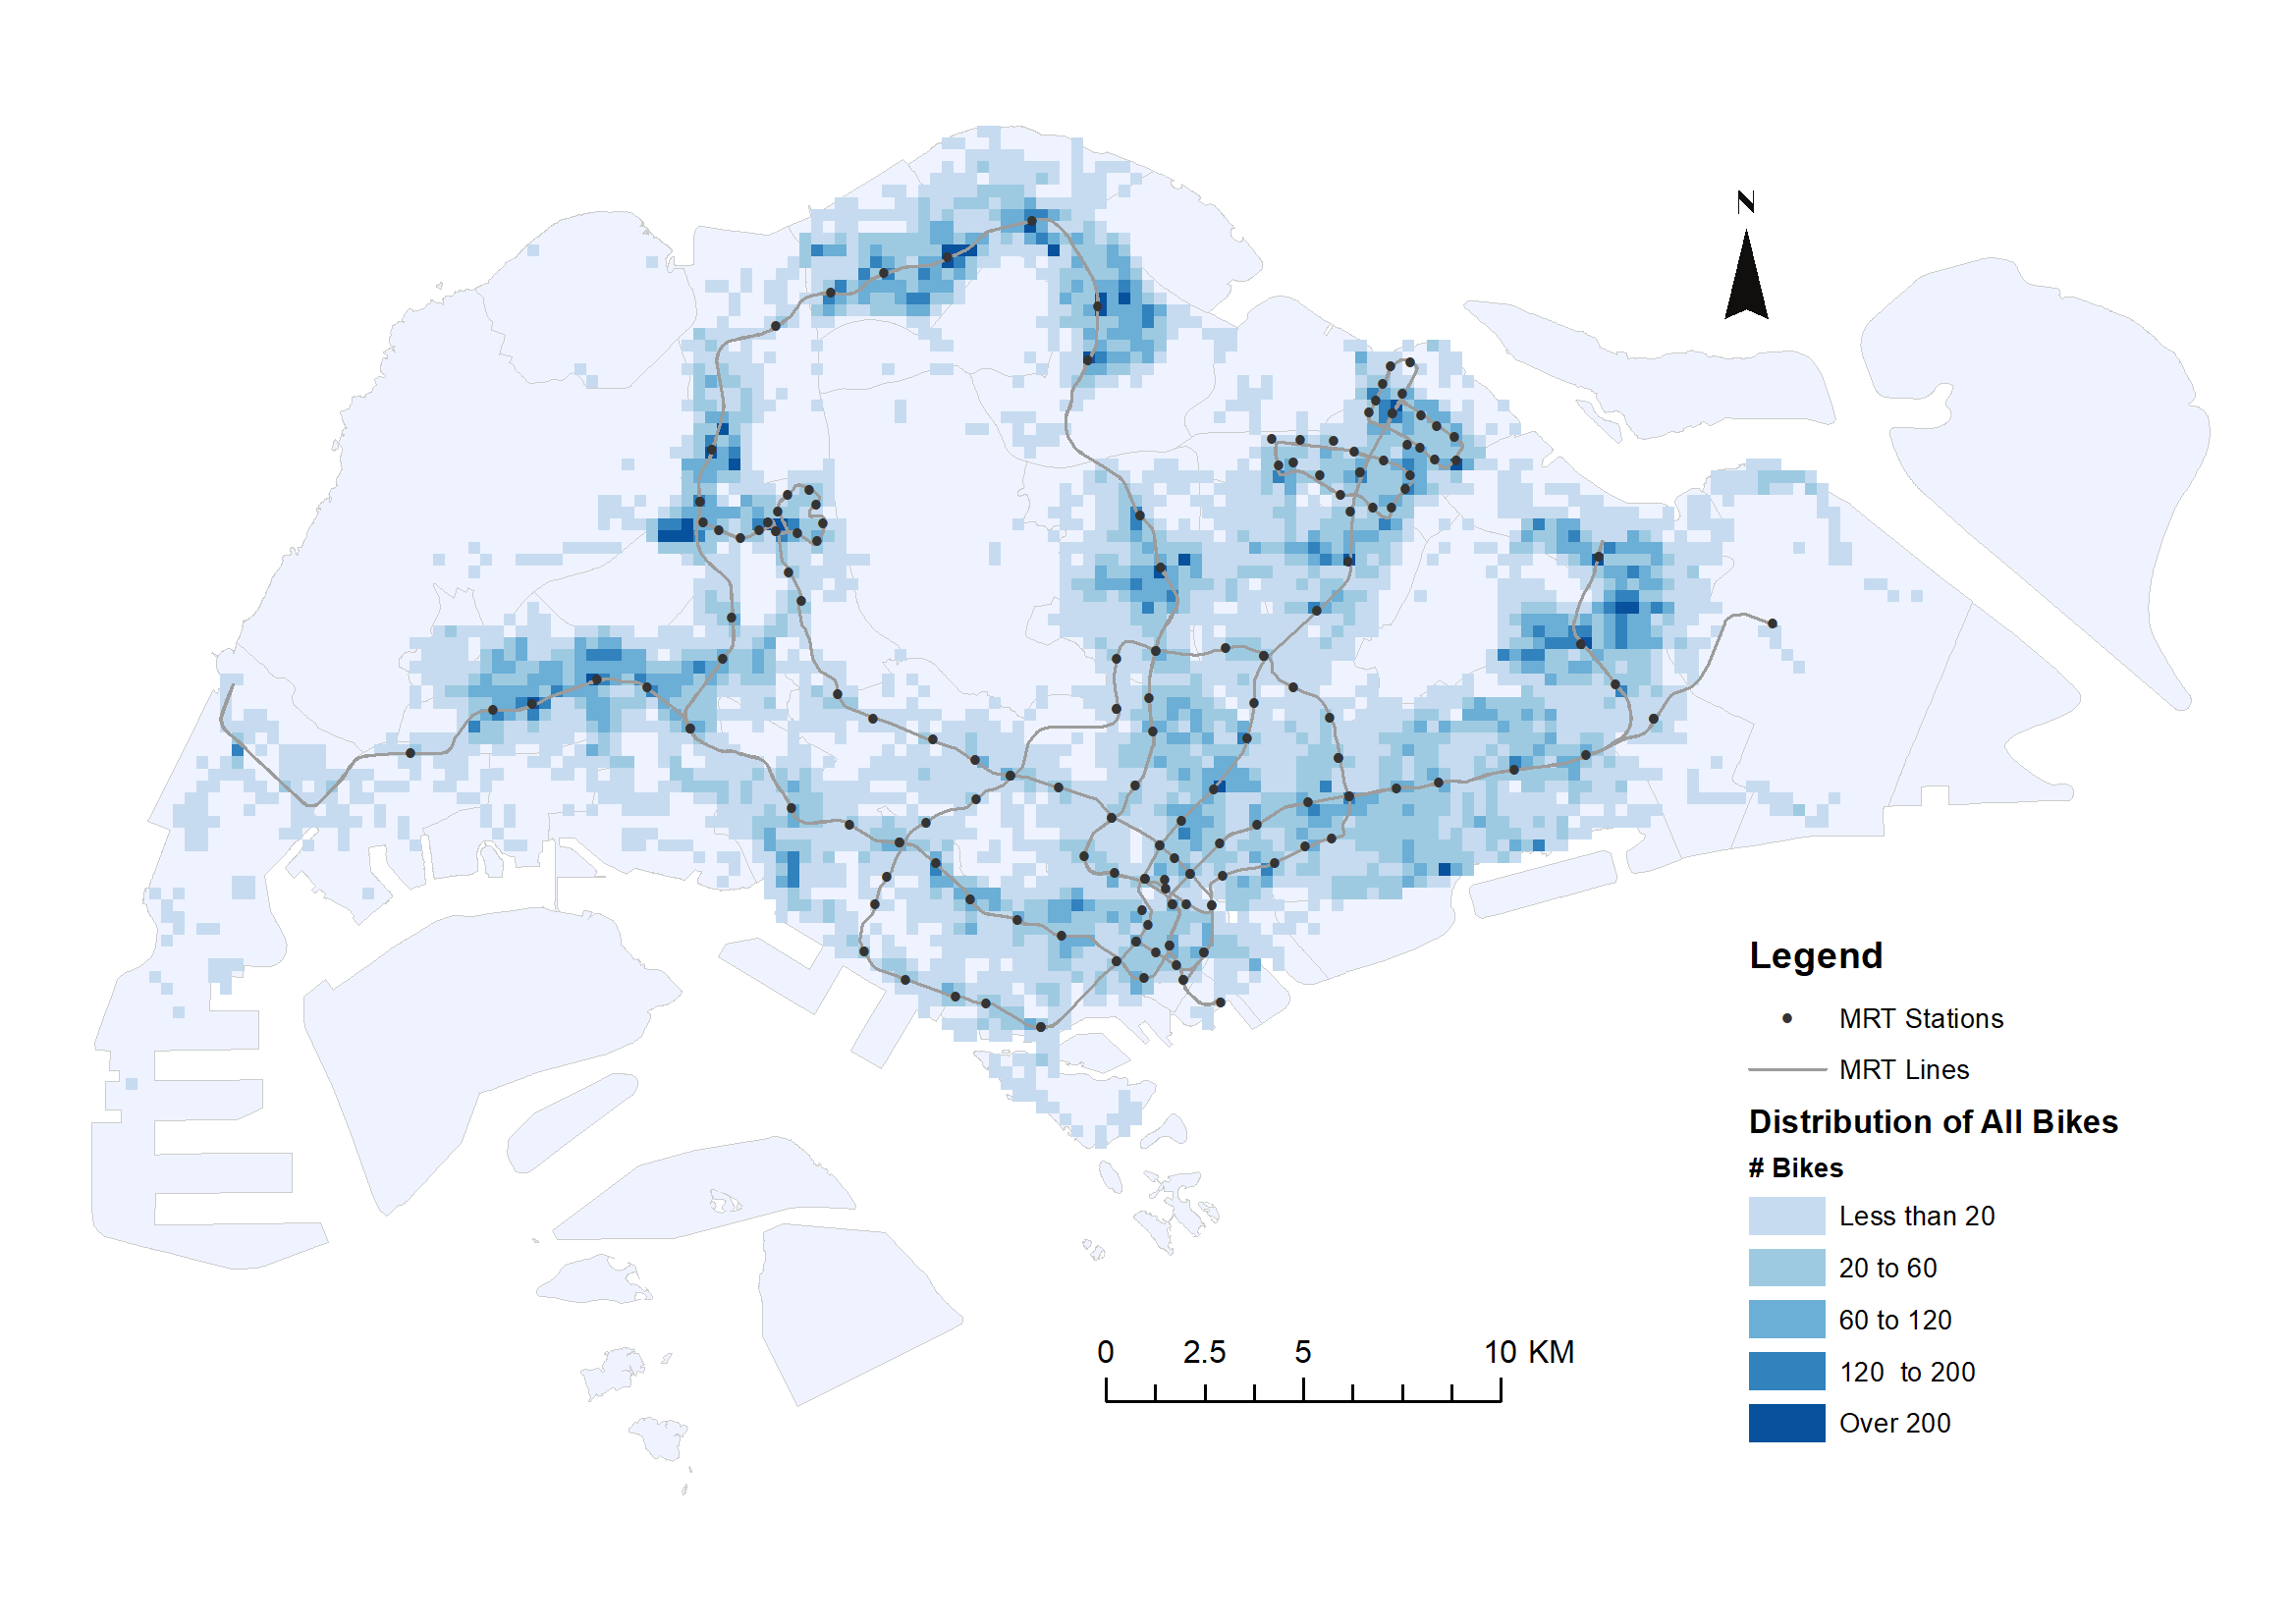
\includegraphics[width= 0.9 \textwidth]{figures_main/spatial_distribution_aday.png}
	\caption{共享单车日分布}
	\label{spatial_aday}
\end{figure}

图\ref{spatial_unused}展示了10月内超过一周没有被使用的车辆比例分布,这个比例可以视为显示该区域中单车过度投放程度的指标。从图\ref{spatial_aday}、图\ref{spatial_unused}两张图中可以很直观的看出,高过度投放程度的区域和高投放量的区域是互补的。除此之外,过度投放程度比较高的区域分布在远离地铁站的区域。这些现象证明单车并没有合理分布,不合理的分布导致了不充分的使用,所以在这个系统中,将单车从那些地利用率的区域调度到需求更高的区域是十分必要的。

\begin{figure}[H]
	\centering
	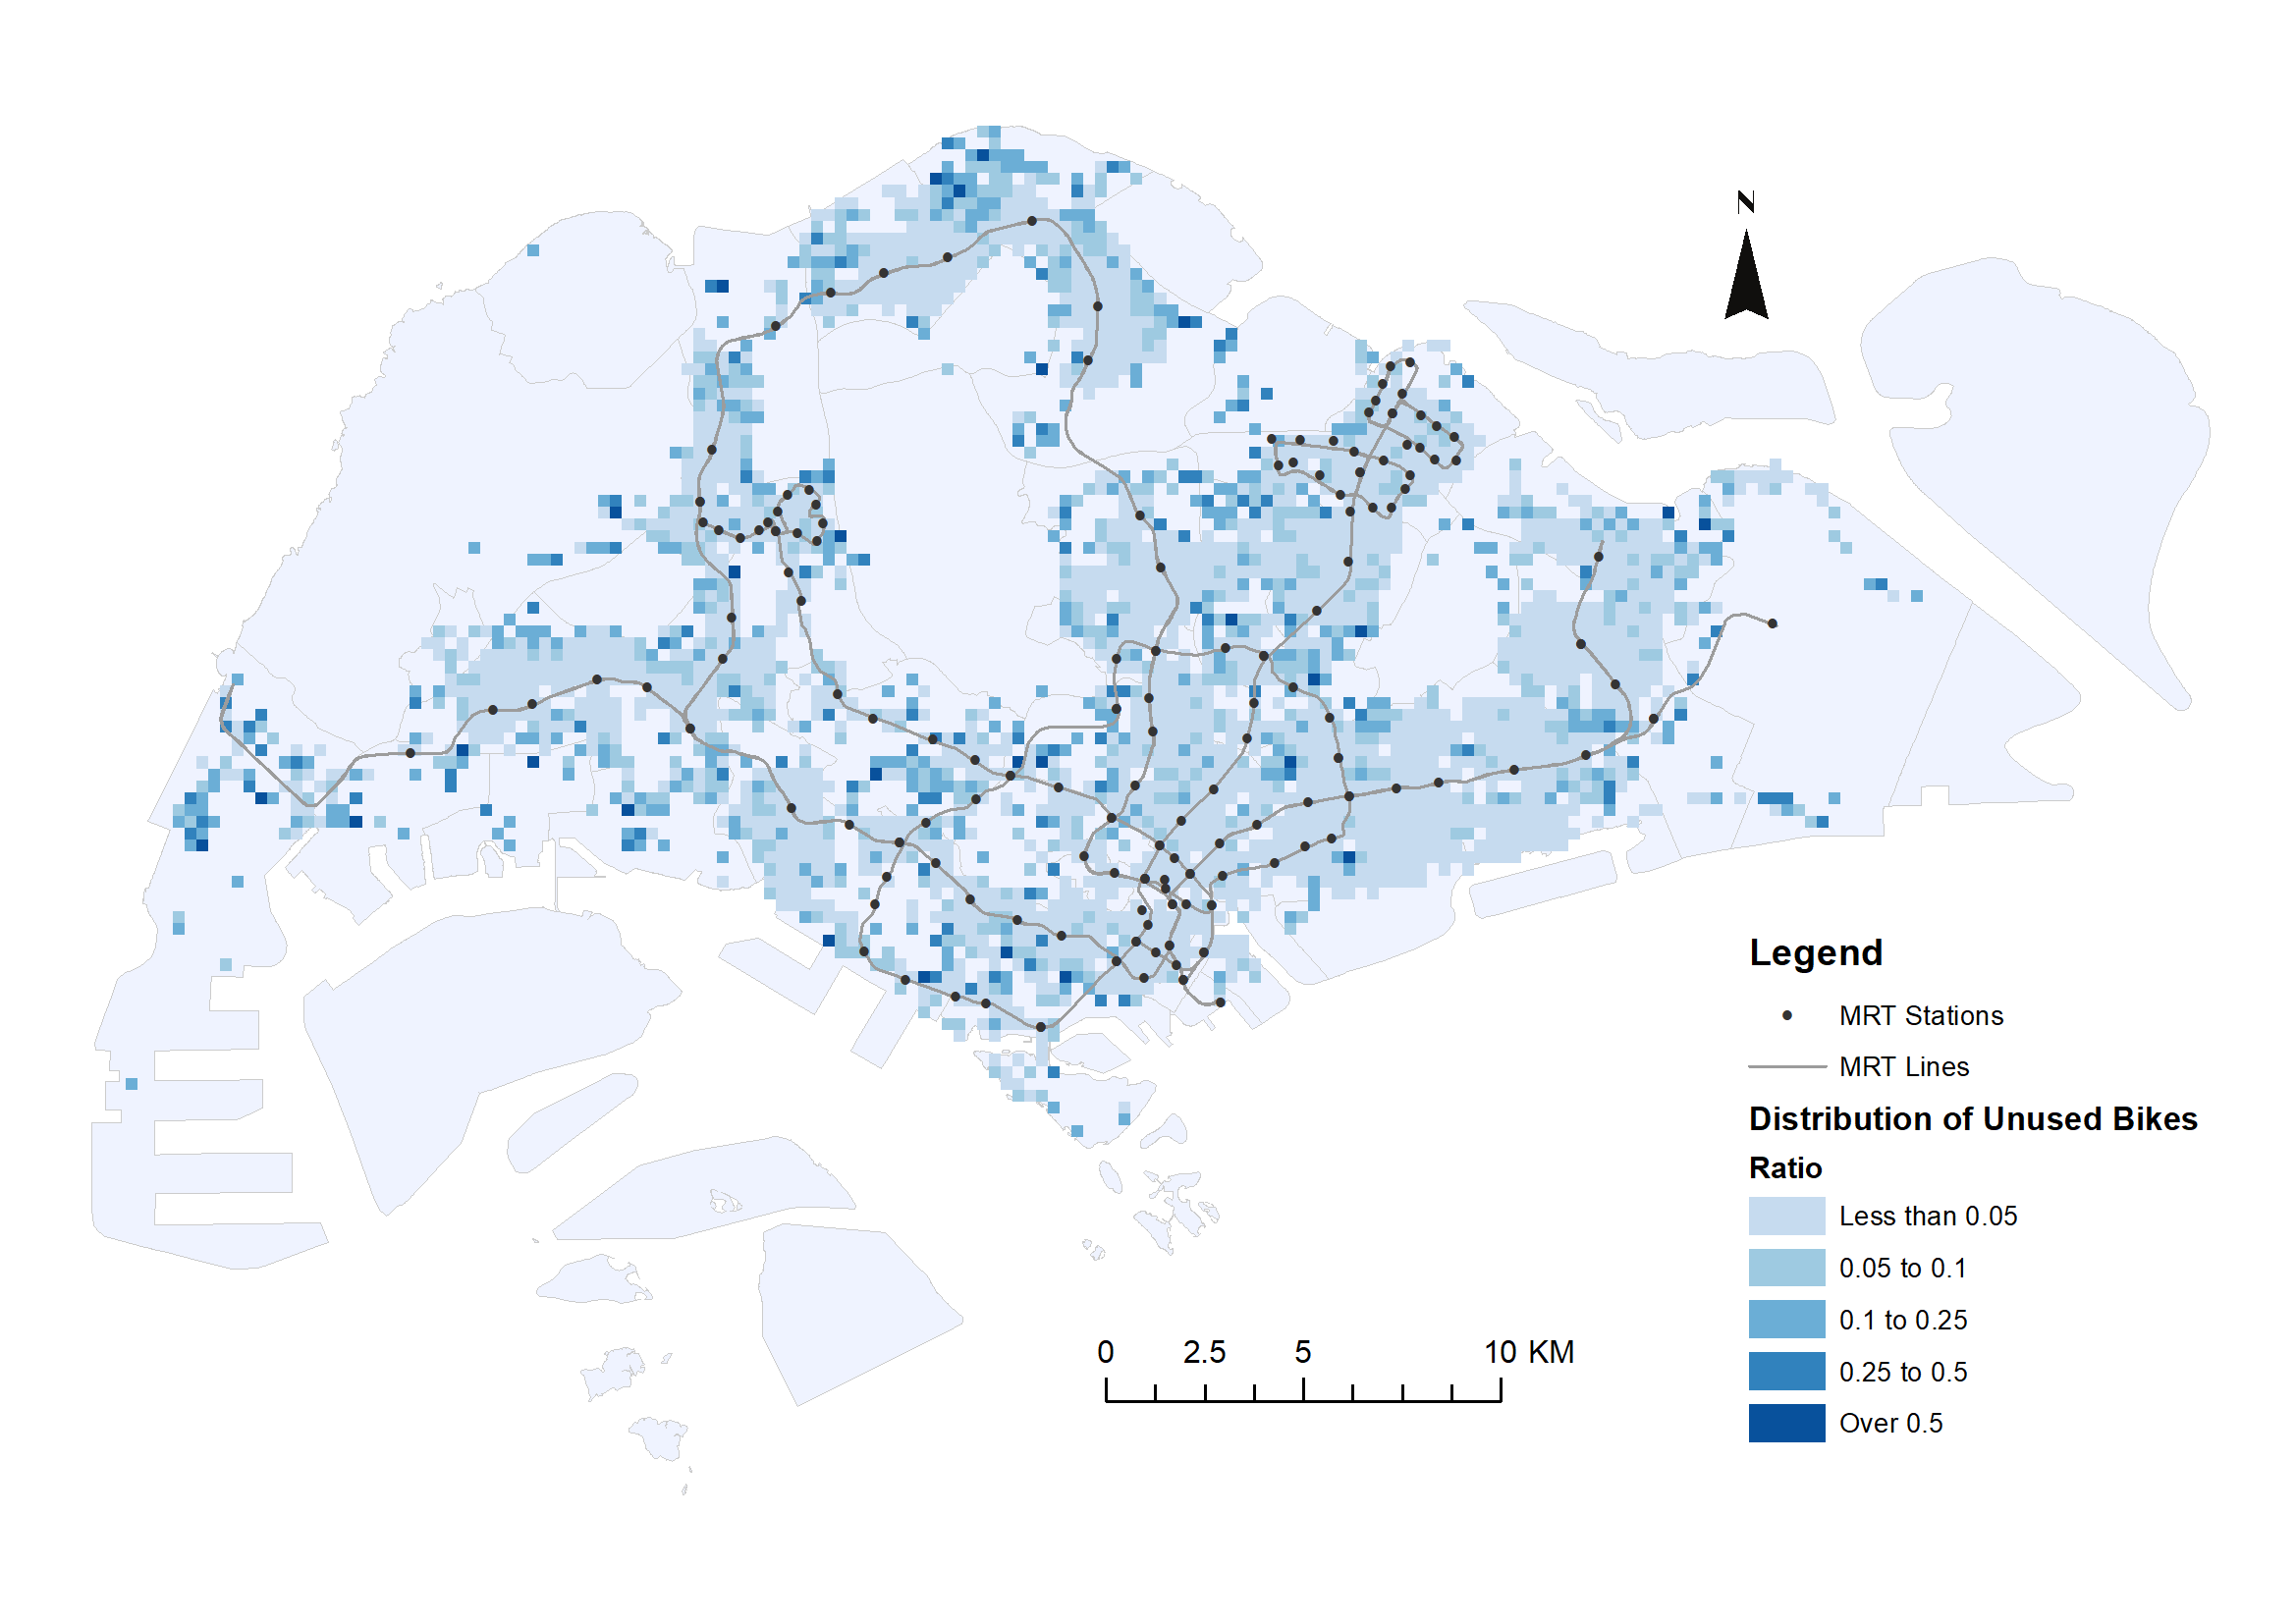
\includegraphics[width= 0.9 \textwidth]{figures_main/unused_spatial_distribution_ratio.png}
	\caption{未使用车辆空间分布}
	\label{spatial_unused}
\end{figure}

在共享单车系统中,调度已经被广泛用于解决在单车数量有限的情况下,不同地区间单车分布不平衡造成的单车利用率低的问题。在之前的研究中,很多学者已经提出了许多用于指定单车调度策略的方案,其中既包括早期的有桩共享单车系统,也包括新式的无桩的单车系统。但事实上,共享单车的有桩和无桩性质在学者们的研究过程中并没有显示本质区别,因为即使在无桩共享单车的建模过程中,研究者们通常也需要将空间连续变量离散化来表示某位置停靠的单车数量,否则问题的规模将会无限大,所以在有桩和无桩单车建模过程中,最显著一个区别是桩的数量是否是系统中单车分配的限制条件。在无桩共享单车系统中,不同单车停放点可以看作没有数量约束的停车桩。

\section{研究概况}
过去几十年来,已有大量研究着眼于对于传统的有桩共享单车系统的调度问题分析。由于停车站的占用率和单车的可用性代表着系统的服务水平已经单车分布的合理性,过去的大部对于有桩共享单车系统的研究都会将停车桩的占用率作为系统服务的一个评价指标。过去的研究总结起来,以调度的动态性划分,过去对于共享单车调度问题的研究可以大致分为两大类:\par
\begin{enumerate}
	\item 只在夜间发生的静态调度(忽略在调度过程中消费者的使用对于单车分布的影响)
	\item 动态调度(将消费者的使用也纳入考虑范围的运营时间内调度)
\end{enumerate}

有关以上的两类调度问题的研究通常关注以下几点问题:
\begin{enumerate}
	\item 需求预测
	\item 车辆路径规划
\end{enumerate}

过去的大部分研究都以路径规划问题的视角考虑调度问题。

由于静态调度问题并不考虑消费者的使用对于调度计划的影响,所以在静态调度相关的研究中,大部分研究者都不会讨论需求预测这一步。而且正如前面提到的,共享单车系统通常涉及到的区域范围广,所以问题规模通常很大,这就导致一部分研究者相比于系统建模过程更加关注寻找更高效的模型求解算法,所以这一类的研究通常旨在为调度模型提供高效且使用的求解算法。例如,对于调度问题,就有学者提出过用Benders分解扩展传统的分支定界\cite{erdougan2015exact}、混合大规模临域搜索\cite{pal2017free}、松弛算法\cite{chemla2013bike}这些算法进行求解。除了在传统的确定性混合整数规划模型的基础上进行改进,启发式算法在求解大规模问题中也运用广泛\cite{ho2014solving,forma20153}。这些启发式算法既有旨在在求解阶段对求解进行加速的,也有在问题分析层面对原问题进行分解的。除了直接从算法层面对求解进行改进,一些研究者还从不同的角度理解调度问题进行建模,利用旅行商问题的建模思路对问题进行抽象\cite{chemla2013bike},此研究与传统的以注消费者满意度和调度成本为优化目标不同的是,目标函数是找到可用单车的方便程度,所有未被满足的需求和调度花费的时间的加权平均值。

虽然静态调度在建模和求解上都更简单,也更易实施,但是对于大部分的城市而言,一天中总是存在高峰和平峰时段,对于单车的需求也就同样存在高峰与平峰。在高峰时段,不同站点间的共享单车需求具有高度的不平衡性,高峰时段过后也很可能会导致单车分布不符合下一高峰的需求。在这种情况下,动态调度是必要甚至是必须的。由于在动态调度中,需求是不可或缺的模型输入,所以在有关动态调度研究中通常也会对需求分析进行讨论。需求分析的方法很多样,有利用马尔可夫过程对系统状态转移进行建模,用以刻画系统中需求的产生和变化规律的\cite{schuijbroek2017inventory},也用利用仿真模拟消费者的期望起终点选择的\cite{caggiani2013dynamic}。无论是利用马尔可夫还是仿真模拟,这些方法都充分考虑了需求产生的原理及其不确定性。为了得到更加弹性、能适应更多现实情况的需求预测方法,有一些研究者对需求和环境、社会因素之间的联系进行了细致的分析。这些因素通常包括温度、天气情况、距离、交通状况等\cite{frade2014bicycle,faghih2014land}。

除了以上希望通过对共享单车需求的产生过程进行细致刻画和分析对共享单车需求进行预测,还有一些研究关注如何利用历史数据对未来需求进行直接预测。具体方法主要集中在线性回归、机器学习和决策树三部分,其中使用线性回归或广义线性回归进行需求预测使用的最为普遍。

这一类型中最早的研究为基于单点的共享单车需求预测。Kaltenbrunner等在2010年提出了一种完全基于同期历史数据的需求预测方法\cite{kaltenbrunner2010urban},通过求过去同一时间段每个站点进出单车数量的变化率,可以求出连续时间内任意时刻站内共享单车的数量,从而决定单车是否过饱和或欠饱和。其它的一些研究集中于通过定义时间、环境(主要是天气)不同的变量表示利用线性回归确定参数从而进行需求预测。在线性回归前往往需要对时间、天气状况这样的变量进行定义和处理,由于难以保证变量间的独立性以及时间、天气与需求间的线性关系,这一类直接回归的模型准确度往往较低。所以在此基础上,Shen.Y 等在对需求影响因素分析的基础上对变量进行了’spatial log’的非线性处理,再利用线性回归求解,结果也证明了这种方法相比直接线性回归具有更高的精确性\cite{shen2018understanding}。由于线性回归出色的可解释性和可以接受的精确度,很多研究都采用这种方法作为需求预测的基础。当然,以上这些模型都假设了单车需求能通过一个具体的函数进行预测,但是在现实生活中,需求的产生往往十分复杂,且具有高度随机性,所以基于机器学习\cite{xu2020hybrid}或基于决策树\cite{ve2020rule}的需求预测研究也因其更高的精确度得到越来越多的研究,但相应的计算成本也更高。

随着站点间需求的相关性和单车需求的动态程度越来越显著,人们逐渐意识到,基于单点的需求预测准确度较低的一个重要原因就是它忽略了需求的不确定性与动态性。所以在此基础上,很多研究者提出了基于“群”的需求预测方法\cite{chen2016dynamic,hulot2018towards},通过站点间需求的相似性先将站点划分为站点群,从而缩小问题规模,再预测群之间的单车流动关系。相比于直接利用线性回归进行需求预测,这种研究方法需要先自定义场景和指标划分站点类型,所以需要的数据种类也更多,除时间和天气状况外,可能还需要额外的社会事件乃至交通状态信息。

近年来,随着无桩共享单车系统的快速发展,对于无桩共享单车调度问题的研究也得到了越来越多的关注。然而,相比于已经发展了几十年的有桩共享单车系统而言,无桩共享单车系统的可用数据以及相关研究基础更少,所以仍缺乏对于无桩共享单车系统调度问题的全面讨论和升入研究。但值得注意的是,已经有一些学者在关注对于无桩共享单车系统特点的讨论\cite{shen2018understanding,li2019operating,xing2020exploring}。基于用户的调度在无桩共享单车调度方法的讨论中也得到了进一步发展。类似的研究有助于促进对调度问题进行更深入、更多样化的探讨。

对于调度问题的研究思路已经越来越突破传统路径规划问题的约束。在动态调度问题的研究中,除了与静态调度相似的采用路径规划作为建模基础的分析思路外,还有一些学者提出了利用奖励机制作为调度手段的方法\cite{fricker2016incentives,ghosh2017incentivizing}。这些研究仔细分析了消费者选择起终点的过程,并基于此给出设置奖励机制鼓励消费者从期望出发站点周围的站点取车或者在期望目的站点周围的站点还车的方法。具体的,有学者通过训练新的强化学习网络解决调度问题,这个网络设计的目的就在于构建一套最优定价算法,激励消费者在高需求区域需要用车时选择在附近区域取车以提高系统的服务水平\cite{pan2019deep}。在此基础上,另一些学者考虑了激励消费者不要在停车车辆过多区域还车的机制\cite{duan2019optimizing,ji2020does}。除了改变调度主体之外,还有学者提出了在更大尺度上考虑调度问题二点思路,比如首先构建一套将研究区域进行动态聚类的方法,将研究区域划分为一个个分区域,在这些区域间讨论调度问题将能大大降低问题规模\cite{caggiani2017dynamic}。

\section{本文的工作框架}
本文将首先对共享单车需求预测的方法进行讨论,并依据现有的数据情况选用最适宜已有数据的需求预测方法。在此基础上,构建一个从有桩共享单车网络中衍生出的用于解决单车调度的网络流量模型,结合从新加坡得到的共享单车实际使用数据以及前述需求预测模型,对调度模型进行了测试检验,证明其合理与有效性。之后,为了加深对不同单车数量、调度卡车数量等因素对收益的影响的理解,利用模型与数据对这些因素进行敏感性分析。最后,对共享单车运营商和政府有关部门提出了一些管理商的建议,以期在保证共享单车系统持续盈利能力的基础上,为社会公众提供更加便捷的共享单车服务。

本文旨在提出一套完整的调度设计流程,从需求预测,到模型的构建,为实际调度计划的制订提供理论支撑。同时为了加深对于共享单车网络运营的理解,利用模型进行网络中各项因素的敏感性分析,以期对共享单车网络的更高效运营提供参考的切入点,使运营商在保证盈利的情况下有能力提供更好的出行用户服务。

以上讨论的调度建模思路和方法最终给出的都是具体到时间的确定性调度方案,适用于在网络运行过程中制定具体的调度计划。近两年来,部分研究者提出一种新的建模方法:基于网络排队的建模方法。Rick和Marco已将这种方法用在网约车调度系统中\cite{zhang2015queueing}。在这个系统中,用户为服务台,网约车为被服务者,模型求解可以得到网约车网络中需要的调度员数量和调度频率。这种模型构建方式得到的结果对运营前共享单车系统的车辆部署、调度用车辆部署有借鉴意义,Maleki Vishkaei等就在共享单车网络中利用网络排队模型进行了最佳站点容量计算以匹配各站点的需求,从而达到减少调度需求的目的\cite{vishkaei2020balancing}。

\clearpage

\chapter{需求预测}
在单车调度模型中,站点间的需求通常是需要预先知道的输入条件。在现实生活中,制订调度计划通常是在调度需求真正发生前,即需要先对未来可能有的需求进行预测才能利用模型进行有效求解。本节将首先对单车需求预测的几种常用方法进行总结,并根据已有数据在这些方法上的测试效果,选取最适合本文使用数据集的预测模型,为之后的数值实验提供支撑。
\section{线性回归}
线性回归是一种简单的预测模型,由于其结果的高度可理解性,被广泛运用在共享单车的需求预测中。线性回归的表达式如下:
\begin{align}
	y = \beta_{0}+\beta_{1}x_{1}+\beta_{2}x_{2}+...+\beta_{n}x_{n}
\end{align}
\noindent
虽然线性回归存在每个变量对结果的影响可以通过线性回归的结果系数直接表示的优点,但是线性回归存在以下突出问题:
\begin{enumerate}
	\item 线性回归假设因变量服从特定自变量下的高斯分布。很多实际问题显然不符合这个假设,例如在共享单车需求预测中,共享单车的需求量恒为非负数,而服从高斯分布意味着预测结果可能为负数值。
	\item 线性回归假设自变量相互独立。在共享单车需求预测中,“天气”和“温度”是两个常被考虑的自变量,而天气和温度显然并非完全独立的变量。
	\item 线性回归假设了每个自变量和因变量间的线性关系。现实世界中的大部分问题都不是线性的。
\end{enumerate}

由于以上问题都涉及到对问题定义的理解这个本质问题,所以通常线性回归在复杂问题中并不能产生令人信服的解释。

\section{广义线性回归(GLM)}
正如上一节中提到的,线性回归总是假设变量与结果间的线性相关关系,而现实中的问题往往具有高度的非线性特性。为了使线性回归能够适应这一点,研究者们提出了广义线性回归(GLM)的概念。广义线性回归本质上就是为自变量与因变量间的映射关系加上一层非线性函数变换,假设这个函数为$f$,广义线性回归的表达式可以表示为:
\begin{align}
	f(x) = \beta_{0}+\beta_{1}x_{1}+\beta_{2}x_{2}+...+\beta_{n}x_{n}
\end{align}

接下来要讨论的单车需求特别是OD对之间的需求具有一定的特征,即数据集中在较小值并且高度分散,有这种特征的数据可以被称为计数数据。计数数据存在的领域很广泛,比如事故发生次数,某种疾病的发病次数等。由于与一般的随机分散的数据有明显的特征差异,计数数据有一套相应的方法论进行分析。在道路风险评估领域,通常用泊松回归或类泊松回归解决这一类问题\cite{mannering2014analytic}。泊松回归也是广义线性回归的一种,它的连接函数为以自然对数为底数的对数函数,并假设因变量服从泊松分布。由于泊松回归还有均值等于方差的假设,而现实中的数据很多情况下都不满足这个条件,所以在泊松回归的基础上,还衍生出了负二项回归、零膨胀泊松回归等模型,这些模型更适用于过度分散或零数据过多的真实数据集。

\section{分类算法}
具有计数特征的数据除了可以被视为计数数据外,还可以当作类别数据处理\cite{lukusa2020horvitz}。对于分类数据处理常用的分类算法包括logistic回归、决策数分类、KNN等,其中logistic回归只适用于二分类问题,而具体采用哪一种分类算法需要根据预测逻辑和数据情况选择。这些分类算法已经具有完备的理论基础,并且在分类问题研究领域已经有了广泛的运用。

还有一类分类算法是基于深度学习的分类算法,这类算法具有处理大规模数据以及高非线性拟合度的优点,是近年来广泛运用于数据处理的一种有效算法。但由于本文不经关注预测结果,也关注结果的可解释性,而深度学习网络的参数多,可解释性较差,所以本文将不对深度学习进行讨论。

\section{单车需求预测}
由于具有计数数据特征,对于单车需求的预测可以尝试类泊松回归的方法;对单车需求预测的基本逻辑是寻找与需要预测的状况最相近的历史状态,即相似的时间段和环境、社会条件下可能产生的单车需求,所以也可以用KNN分类算法进行预测。建模过程分为数据准备、数据集划分、模型训练、模型测试这几个阶段。以下先讨论数据准备过程,再分别讨论这两个方法得到的最终结果。

\subsection{数据准备}
本文使用的原始数据为单车使用订单数据,包括的字段有\{车辆ID,时间戳,起始精度,起始纬度,终止精度,终止纬度,骑行时间,骑行距离\},在需求预测阶段,对原始数据进行如下处理:
\begin{enumerate}
	\item 利用四分位法和骑行时间,骑行距离处理异常订单数据。
	\item 以一小时的时间间隔划分时间片,将订单中的起止时间拆分为起止日期,时间片编号这两个字段
	\item 以起止土地块编号、出发时间为分类字段统计对应时间片内,从对应起点到终点的单车数量,次时数据字段变为\{起始cell编号,终止cell编号,日期,时间片编号,单车使用数量,起终点距离,起始土地块熵,终止土地块熵\}。
	\item 在每条记录上添加起止土地块间距离、气质土地块静态信息(代表土地块利用情况的信息)字段
	\item 从新加坡开源数据网站https://data.gov.sg/上获取分析时段内新加坡各个监测站测得的温度和降雨信息,并通过克里金插值,得到每个起始土地块在对应时刻的温度和降雨情况,并入每条记录中。
\end{enumerate}

经过以上处理,最终用作建模和预测的数据集包含的字段为\{起始cell编号,终止cell编号,日期,时间片编号,单车使用数量,起终点距离,起始土地块熵,终止土地块熵,温度,降雨\}。由于无论是采用负二项分布还是KNN,自变量的尺度都会对系数或距离的计算产生影响,所以在训练前还需要对自变量字段进行标准化处理。

单车使用具有周期性特征,例如每个工作日间的使用特征相似,所以在划分训练集和测试集阶段,并不随机划分,而是在四周的数据中挑选前三周作为训练集,后一周作为测试集。另外,周末和工作日的单车使用具有差异性,所以在预测时,将工作日和周末分别用两个模型进行预测。

\subsection{类泊松回归}
处理完成的数据中单车使用数量字段的值得统计图如图\ref{usecount}所示。从图中可以看出,两站点间得单车使用数量基本集中在6以下得较小值,且从分布上来看符合2.2中提到的计数数据的分布特征。这个字段的均值为0.18,方差为0.56,属于过度分散的数据集,所以接下来利用负二项分布模型对需求进行预测。
\begin{figure}[H]
	\centering
	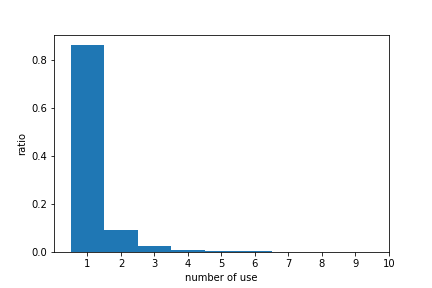
\includegraphics[width= 0.7 \textwidth]{figures_main/counthist.png}
	\caption{单车使用次数统计}
	\label{usecount}
\end{figure}

负二项分布对均值和方差间关系的假设为:
\begin{align}
variance = mean + \alpha \cdot mean^{n}
\end{align}
本文取$n$为2,即采用NB2型负二项分布进行训练和预测。

在建模过程中,当将时间、起终点间距离、起终点土地利用情况、温度、降雨都作为自变量输入负二项分布时,由于降雨量的方差太小,模型会将自变量矩阵判断为不可逆,所以在负二项回归中删去降雨列,得到的工作日拟合结果如表\ref{weekday}所示。工作日用于训练的数据共有2676319条,结果$r^2$值为0.001。
\vspace{3mm}    %空一行
\begin{table}[H]
	\centering	
	\caption{工作日}
	\label{weekday}
	\renewcommand\arraystretch{1.5}	%行间距放大为1.5倍
	\begin
	{tabular}{p{17mm}<{\centering} p{10mm}<{\centering} p{10mm}<{\centering} p{15mm}<{\centering} p{10mm}<{\centering} p{10mm}<{\centering} p{10mm}<{\centering}}
		\toprule[2pt]
		variable & Coef & std err & z & p>|z| & 0.025 & 0.975 \\
		\midrule[1pt]
		const & -1.7135 & 0.002 & -1032.607 & 0.000 & -1.717 & -1.710 \\
		hour & -0.0229 & 0.002 & -13.089 & 0.000 & -0.026 & -0.019 \\
		distance & 0.0474 & 0.002 & 29.404 & 0.000 & 0.044 & 0.051  \\
		entropystart & 0.0013 & 0.002 & 0.806 & 0.420 & -0.002 & 0.005 \\
		entropyend & -0.0073 & 0.002 & -4.402 & 0.000 & -0.011 & -0.004\\
		temperature & 0.0712 & 0.002 & 41.338 & 0.000 & 0.068 & 0.075 \\
		alpha & 1.8021 & 0.009 & 193.343 & 0.000 & 0.068 & 0.075 \\
		\bottomrule[2pt]
	\end{tabular}
\end{table}
\vspace{3mm}

从表格中可以看出,温度和距离对需求的影响较大。在工作日,距离、温度、起点处土地利用熵系数为正,说明起终点间距离越大,温度越高,起点繁华程度越高,单车的使用数量越多。由于义顺区的面积比较小,大致为三公里乘四公里,所以在这个区域内,共享单车能够骑行的最大距离也就在三只四公里,在共享单车比较适宜的骑行距离之内,所以产生需求的两土地块间距离对于义顺区的尺度来说比较大,从而使得结果体现出距离越大,需求越高的情况。

利用以上模型对664107条测试集数据进行测试,得到预测结果整体的准确度为51\%。
\begin{comment}
\vspace{3mm}    %空一行
\begin{table}[H]
	\centering	
	\caption{工作日}
	\label{weekday_score}
	\renewcommand\arraystretch{1.5}	%行间距放大为1.5倍
	\begin
	{tabular}{p{17mm}<{\centering} p{10mm}<{\centering} p{10mm}<{\centering} p{10mm}<{\centering} p{10mm}<{\centering} p{10mm}<{\centering} p{10mm}<{\centering} p{10mm}<{\centering} p{10mm}}
		\toprule[2pt]
		需求量 & 0 & 1 & 2 & 3 & 4 & 5 & 6 & >=7 \\
		\midrule[1pt]
		数据量/条 & 587288 & 64799 & 7313 & 1998 & 879 & 453 & 281 & 556 \\
		预测正确/条 & 328344 & 13135 & 194 & 70 & 30 & 8 & 4 & 0 \\
		准确度/\% & 56 & 20 & 3 & 4 & 3 & 2 & 1 & 0 \\
		\bottomrule[2pt]
	\end{tabular}
\end{table}
\vspace{3mm}
\end{comment}

对周末数据进行和以上相同的分析后得到的结果分别如表\ref{weekend},\ref{weekend_score}所示。周末模型拟合结果的$r^2$值为0.02,相比工作日高。从表\ref{weekend}可以看出,周末的终点熵值对需求的影响比工作日更加明显,且起终点的熵值越大,需求越大,这说明在周末消费者常活动在较繁华的区域周围。
\vspace{3mm}    %空一行
\begin{table}[H]
	\centering	
	\caption{周末}
	\label{weekend}
	\renewcommand\arraystretch{1.5}	%行间距放大为1.5倍
	\begin
	{tabular}{p{17mm}<{\centering} p{10mm}<{\centering} p{10mm}<{\centering} p{15mm}<{\centering} p{10mm}<{\centering} p{10mm}<{\centering} p{10mm}<{\centering}}
		\toprule[2pt]
		variable & Coef & std err & z & p>|z| & 0.025 & 0.975 \\
		\midrule[1pt]
		const & -1.8374 & 0.003 & -625.403 & 0.000 & -1.843 & -1.832 \\
		hour & 0.2621 & 0.003 & 80.209 & 0.000 & 0.256 & 0.268 \\
		distance & 0.1035 & 0.003 & 39.120 & 0.000 & 0.098 & 0.109  \\
		entropystart & 0.0216 & 0.003 & 7.605 & 0.000 & 0.016 & 0.027 \\
		entropyend & 0.0176 & 0.003 & 6.225 & 0.000 & 0.012 & -0.023\\
		temperature & 0.2579 & 0.003 & 95.537 & 0.000 & 0.253 & 0.263 \\
		alpha & 1.5884 & 0.015 & 105.146 & 0.000 & 1.559 & 1.618 \\
		\bottomrule[2pt]
	\end{tabular}
\end{table}
\vspace{3mm}

在测试集上,周末预测的整体准确度为29\%,明显低于工作日,这说明周末需求的产生比较随机。
\begin{comment}
\vspace{3mm}    %空一行
\begin{table}[H]
	\centering	
	\caption{周末}
	\label{weekend_score}
	\renewcommand\arraystretch{1.5}	%行间距放大为1.5倍
	\begin
	{tabular}{p{17mm}<{\centering} p{10mm}<{\centering} p{10mm}<{\centering} p{10mm}<{\centering} p{10mm}<{\centering} p{10mm}<{\centering} p{10mm}<{\centering} p{10mm}<{\centering} p{10mm}}
		\toprule[2pt]
		需求量 & 0 & 1 & 2 & 3 & 4 & 5 & 6 & >=7 \\
		\midrule[1pt]
		数据量/条 & 667579 & 110109 & 12215 & 3143 & 1235 & 568 & 313 & 720 \\
		预测正确/条 & 251604 & 24257 & 1229 & 195 & 47 & 13 & 8 & 3 \\
		准确度/\% & 38 & 22 & 10 & 6 & 4 & 2 & 3 & 0.4 \\
		\bottomrule[2pt]
	\end{tabular}
\end{table}
\vspace{3mm}
\end{comment}

\subsection{KNN}
由于共享单车使用规律存在周期性特征,所以对共享单车进行需求预测的逻辑为期望通过寻找相似场景下的历史需求,得到当前场景需求的可能值,这与KNN算法的逻辑是一致的,KNN的预测方法即为找到与待预测点值相近的训练集中的点,利用这些点的情况对待分类点进行预测。

利用KNN得到的在工作日和周末的测试集上的预测准确度分别为87\%,82\%。
\begin{comment}
\vspace{3mm}    %空一行
\begin{table}[H]
	\centering	
	\caption{工作日}
	\label{knn_weekday_score}
	\renewcommand\arraystretch{1.5}	%行间距放大为1.5倍
	\begin
	{tabular}{p{17mm}<{\centering} p{10mm}<{\centering} p{10mm}<{\centering} p{10mm}<{\centering} p{10mm}<{\centering} p{10mm}<{\centering} p{10mm}<{\centering} p{10mm}<{\centering} p{10mm}}
		\toprule[2pt]
		需求量 & 0 & 1 & 2 & 3 & 4 & 5 & 6 & >=7 \\
		\midrule[1pt]
		数据量/条 & 667579 & 110109 & 12215 & 3143 & 1235 & 568 & 313 & 720 \\
		预测正确/条 & 573587 & 2254 & 0 & 0 & 0 & 0 & 0 & 0 \\
		准确度/\% & 85 & 2 & 0 & 0 & 0 & 0 & 0 & 0 \\
		\bottomrule[2pt]
	\end{tabular}
\end{table}
\vspace{3mm}

\vspace{3mm}    %空一行
\begin{table}[H]
	\centering	
	\caption{周末}
	\label{knn_weekend_score}
	\renewcommand\arraystretch{1.5}	%行间距放大为1.5倍
	\begin
	{tabular}{p{17mm}<{\centering} p{10mm}<{\centering} p{10mm}<{\centering} p{10mm}<{\centering} p{10mm}<{\centering} p{10mm}<{\centering} p{10mm}<{\centering} p{10mm}<{\centering} p{10mm}}
		\toprule[2pt]
		需求量 & 0 & 1 & 2 & 3 & 4 & 5 & 6 & >=7 \\
		\midrule[1pt]
		数据量/条 & 849892 & 117832 & 14001 & 3777 & 1531 & 706 & 402 & 889 \\
		预测正确/条 & 690297 & 5897 & 2 & 0 & 0 & 0 & 0 & 0 \\
		准确度/\% & 81 & 5 & 0 & 0 & 0 & 0 & 0 & 0 \\
		\bottomrule[2pt]
	\end{tabular}
\end{table}
\vspace{3mm}
\end{comment}

\subsection{方法比较}
本节将从运行时间、效果和结果的可解释性三个方面对用负二项回归和KNN分类对需求进行预测的方法进行比较。

从运行时间上看,在针对较大训练数据集时,KNN相比于负二项回归具有较快的训练速度,但是其预测速度比负二项回归慢。由于在现实生活中,历史数据集的量往往很大,较快的训练速度可以达到在有限时间内更充分的利用这些数据的目的;在调度问题中需要预测的时间段往往比较固定,可能是一天、一周或一个月,数据量相对较小,所以预测速度稍慢并不会产生太大影响。

从准确度上看,利用KNN进行预测的准确度高于负二项回归。

从结果的可解属性来看,直观上看,上利用负二项分布可以直接得到每个变量的系数,从而可以直接对每个变量对结果的影响进行解释和理解,而利用KNN构建的模型难以做到这一点。

机器学习算法的可解释性之所以重要,是因为人们除了希望获得具有高准确度的模型之外,往往还期望能够通过这个模型对问题的本质进行探究和理解,这种理解有助于模型参数的调优,以及在模型无法很好的解释现象时,对可能的原因进行分析。

虽然机器学习的可解释性可以带来诸多好处,对于大部分高效的机器学习算法而言,想要对其参数进行解释并不容易。例如,在神经网络中有成百上千的参数,由于在神经网络计算过程中的高度非线性性质,我们很难从训练好的神经网络中通过每个参数的值计算对应的自变量的系数,所以很难像诸如线性回归这一类的算法一样直接通过系数值的大小对问题进行解释。

为了解决这个问题,一些学者提出了可解释机器学习的概念。可解释机器学习的方法很多样,Molnar在他的书中对常用的方法进行了总结和解释\cite{molnar2019}。从基本原理上看,可解释机器学习就是试图拆分每个参数对结果的影响,从而衡量这个参数在此问题中所起的作用。接下来本文将采用Shapley值法,对KNN模型进行解释。

Shapely值计算的基本思想为,通过改变一个变量的值,保持其它变量在平均值,计算这个变量改变时结果的改变程度,这个改变程度即代表了这个变量对结果的影响。例如在我们的单车需求问题预测中,假设预测的所有需求的平均值为2,我们需要解释的是,当时间、距离、起终点土地利用情况、温度和降雨共同预测出一个为3的需求时,每个自变量对3和2间的差异,即1,贡献了多少。以时间为例,当计算时间的Shapely值时,首先我们给定一个时间值,从数据集中随机选取除时间以外的其它自变量的值,产生一条新的数据,再利用模型对这条数据进行预测得到需求值;接下来,再从数据集中随机选取时间值代替一开始选定的时间值,再次用模型预测需求。这两次需求的差值即为时间这个变量对结果的贡献量。为了提高计算准确度,重复以上第二步中的采样过程,并对所有过程计算平均值作为最终的Shapely值。

从Shapely值的计算原理中可知,不仅可以计算单个实例的Shapely值,还可以计算模型整体的Shapely值,这两种Shapely值对应的就是可解释机器学习中的局部解释和全局解释。局部解释侧重于分析在单个实例中,各个自变量是如何共同作用产生预测结果的,全局解释则可以帮助人们理解所研究的问题的整体逻辑结构。

对于工作日KNN模型计算的两个实例的Shapely值如图\ref{ex1}、\ref{ex2}所示。从两图中可以看出,对于不同的实例,不同的自变量对结果的影响不同。不过,对于单车需求预测而言,我们并不关系单个预测是如何产生的,更关心的是每个自变量对需求产生的整体影响
\begin{figure}[H]
	\centering
	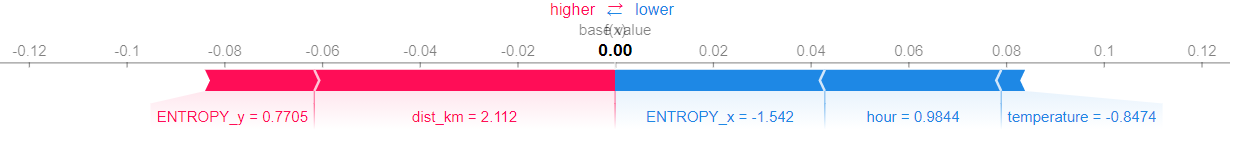
\includegraphics[width= 0.8 \textwidth]{figures_main/ex_weekday1.png}
	\caption{实例1}
	\label{ex1}
\end{figure}

\begin{figure}[H]
	\centering
	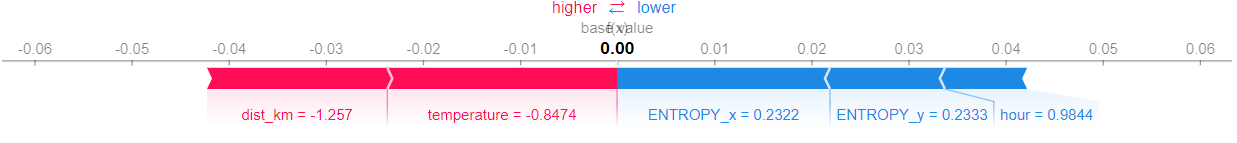
\includegraphics[width= 0.8 \textwidth]{figures_main/ex_weekday2.png}
	\caption{实例2}
	\label{ex2}
\end{figure}

整体Shapely值如下图\ref{weekday_shap1}所示。从图中可以直接看出,距离、时间对预测结果的影响比较大,温度和起终点土地利用情况对预测结果的影响较小,这与之前用负二项回归训练结果中参数的解释是一致的。
\begin{figure}[H]
	\centering
	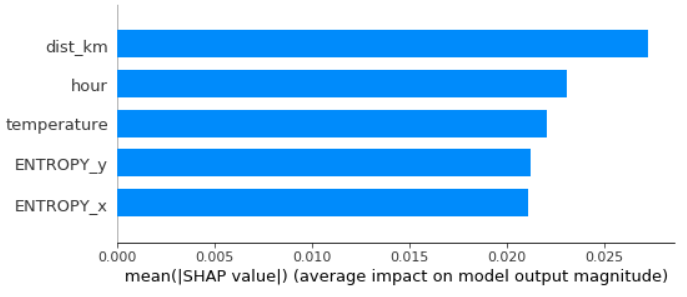
\includegraphics[width= 0.9 \textwidth]{figures_main/shape_weekday.png}
	\caption{工作日Shapely值}
	\label{weekday_shap1}
\end{figure}

下图\ref{weekday_shap2}是对类似图\ref{ex1}、图\ref{ex2}的每个实例的汇总。从图中的分布可以看出,站点间距对预测结果的影响整体为正值,即站点间距使得模型对需求的预测增加;时间对预测结果的影响更偏向负值,这与在利用负二项分布拟合时对结果的分析是相似的。
\begin{figure}[H]
	\centering
	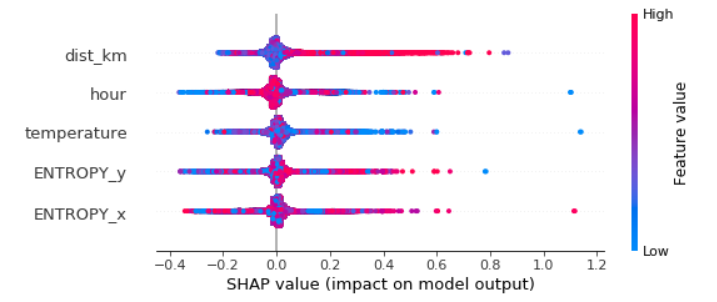
\includegraphics[width= 0.9 \textwidth]{figures_main/shap1_weekday.png}
	\caption{工作日Shapely值}
	\label{weekday_shap2}
\end{figure}
\clearpage

\chapter{调度模型建立}
\section{问题阐述}
在之后的文章中,我们将在动态的共享单车调度系统中利用时空网络模型模拟单车的使用和停放、卡车的调度行为的过程并分析他们对于系统运行结果的影响。由于调度卡车的数量有限,而共享单车的数量往往远大于调度车辆的数量,如果将单车的数量视为离散变量会大大增加模型的求解难度,所以在模型构建过程中,将每辆调度卡车视为独立的个体,即代表卡车数量的变量为整数变量,而将单车视为连续流,即代表单车数量的变量为连续变量。最终得到的模型是一个混合整数优化问题。为了更好的理解建模过程,本节先对建模过程中需要用到的一些符号的含义进行解释说明,具体如表\ref{tab:notation}所示。
\vspace{3mm}    %空一行
\begin{table}[H]
	\centering	
	\caption{符号表示}
	\label{tab:notation}
	\renewcommand\arraystretch{1.5}	%行间距放大为1.5倍
	\begin
	{tabular}{p{15mm}<{\centering} p{10mm}<{\centering} p{70mm}<{\centering}}
		\toprule[2pt]
		变量类型 & 符号 & 释义 \\
		\midrule[1pt]
		集合 & $N$ & 站点(土地块)集合  \\
		集合 & $A$ & 两站点间最近连线集合 \\
		集合 & $T$ & 时间切片 \\
		\midrule[1pt]
		参数 & $c_{ij}^v$ & 从站点$i$运送一辆单车到站点$j$的成本,包括在$i$装载单车和在$j$卸载单车  \\
		参数 & $c_{ij}^u$ & 从$i$到$j$的过程中一辆单车的磨损成本 \\
		参数 & $e_{ij}^d$ & 消费者将单车从$i$骑到$j$需要的费用 \\
		参数 & $a$ & 调度卡车容量 \\
		参数 & $n$ & 系统中的单车总数 \\
		参数 & $r_{ij}^t$ & 在时间片$t$期望将单车从$i$骑到$j$的消费者数量 \\
		参数 & $P$ & 其它固定成本,例如购买单车成本 \\
		\midrule[1pt]
		连续变量 & $b_{ik}^{t,t_k}$ & 在$[t,t_k]$被从$i$运送到$j$的单车数量 \\
		连续变量 & $b_i^t$ & 时间片$t$时停在$i$的单车数量 \\
		连续变量 & $d_{ij}^{t,t_j}$ & 在$[t,t_j]$被消费者从$i$骑到$j$的单车数量 \\
		\midrule[1pt]
		离散变量 & $w_{ik}^{t,t_k}$ & 在$[t,t_k]$从$i$到$j$的卡车数量 \\
		离散变量 & $u_i^t$ & 时间片$t$时停在$i$的卡车数量 \\
		\bottomrule[2pt]
	\end{tabular}
\end{table}
\vspace{3mm}

上表中,$n$代表系统中调度卡车数量,每辆卡车的运载容量为$a$,即一辆卡车一次最多只能运送$a$辆单车。在空间维度上,由于在无桩共享单车系统中并没有固定的车辆停放点,为了表示车辆停放位置,我们需要先将整个共享单车服务区域划分为一些更小的分区,这些分区的划分应以共享单车消费者常用的停车区域为依据,并且能被视为没有停放数量的限制。以下过程中将这些分区称为土地块或站点。$N$代表研究区域中划分的土地块的数量。在时间维度上,需要将连续的时间变量分割为从1到$T$的时间片。$b_i^t$代表在时间片$t$停放在土地块$i$的单车数量,$u_i^t$代表在时间片$t$在土地块$i$等候的调度卡车数量。在定义的这些基础变量的基础上,接下来定义与单车和卡车在不同时间片内移动有关的决策变量如下:
\begin{enumerate}
	\item 在时间片$[t,t_k]$内被调度用车从土地块$i$运送到$k$的单车数量$b_{ik}^{t,t_k}$
	\item 在时间片$[t,t_k]$内被用户从土地块$i$骑到$k$的单车数量$d_{ij}^{t,t_j}$
	\item 在时间片$[t,t_k]$内被从土地块$i$运送单车到$k$的调度卡车数量$w_{ik}^{t,t_k}$
	\item 在时间片$[t,t_k]$内被从土地块$i$空载到$k$的调度卡车数量$u_{ik}^{t,t_k}$
\end{enumerate}

$t$和$t_k$,$t$和$t_j$间的差值由对应OD对间的距离和单车或卡车的速度决定。在模型中,我们还假设调度卡车在站点进行单车搬运操作的时间为一个常数,即这个时间不会随需要搬运的单车的数量变化。虽然这个假设是为了简化模型,但也同时是这个模型的一个局限,不过想要解决这个问题,可以在模型中添加一个表示操作时间的变量。

(start)为了更好的阐述模型的构建逻辑,以下先通过一个小型网络中的例子来描述本文对调度过程的刻画逻辑。图\ref{network_example}展示了一个由三个站点和三个时间切片组成的小型时空网络,图中只展示了站点1在时间片1的单车与卡车流,其它站点同理。流入和流出站点1的单车流由两部分组成:卡车的运送和消费者的使用。相邻两个时间切片下同一站点的单车数量关系就可以由这两部分的流量完全表示。在图\ref{network_example}表示的例子中,从站点1到3的卡车和单车流耗时不同,因为卡车和单车的速度不同。需要特别提出的是,在考虑两站点间的运行时间时,我们只关注站点间的距离,而不关注具体的路线,这意味着无论图中的站点2是否位于站点1和3之间都不会影响模型的最终结果。最后,模型中所有的时间都以时间切片为单位,不足一个时间片的按一个时间切片计。
\begin{figure}[H]
	\centering
	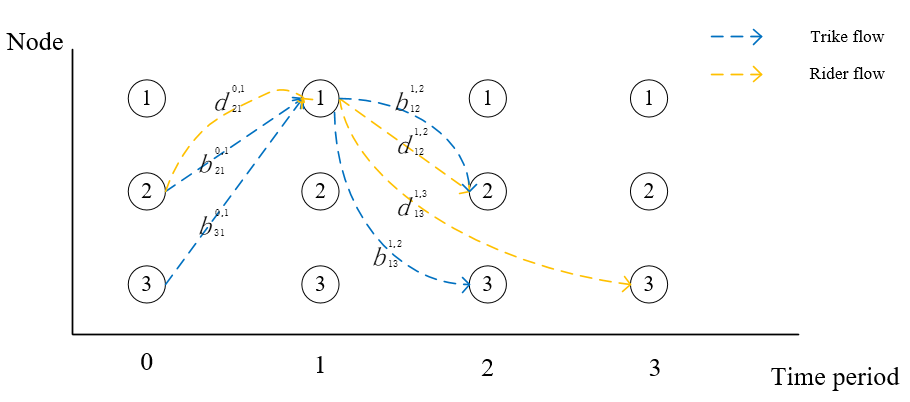
\includegraphics[width=0.8 \textwidth]{figures_main/network_example.png}
	\caption{小型时空网络示例 \\
			 (站点1在时间片1的流入流出)
			}
	\label{network_example}
	\end{figure}

\section{问题抽象与建模}
本节将讨论将实际调度问题抽象成可解的数学模型的过程,我们将提出一个混合整数线性规划模型用于描述和解决单车调度问题。建立这个模型的目的是为了动态的为卡车调度行为提供理论指导,以使得共享单车网络在现有规模下能获得可能的最优收益。模型的目标收益仅指消费者使用共享单车带来的收益与调度成本(包括搬运、运输单车过程中的磨损成本)和卡车调度的成本间的差值。其它成本,如车辆贬值、卡车司机工资等成本更适合在考虑网络长期稳定运营的问题中考虑,且受诸多其它社会因素的影响,所以本模型中并未涉及,本模型只重点关注如何利用有限的卡车和共享单车得到最大的现实收益,最后得到的主要结论是在每个时间片,应在网络中执行什么样的调度操作,具体到卡车应从何处将多少单车调度到何处。

为了尽可能的降低模型构建过程中一些不必要的现实情况造成的建模困难,只关注共享单车调度过程中那些最本质的问题,将模型构建前先做出的假设和简化以及模型使用的网络特点总结如下:
\begin{enumerate}
	\item 整个研究时间段需要被切分为具有相等间隔的时间切片。
	\item 每个OD对间在每个时间切片内的需求都是可以预先预测的。
	\item 每个消费者都可以直接从他们的出发地到达目的地,不需要绕行到其它位置。
	\item 尽管单车和卡车的速度受实时交通状况的影响,但是在模型中,将两者的速度视为可知的定值。
	\item 单车骑行依据使用时间收费,这个费用在确定起终点和速度后就可以直接估计出来。
	\item 共享单车流为连续流,调度卡车流为离散值。
	\item 如果消费者在他们的期望始发点没有找到可用单车,则他们应直接离开。换言之,消费者不会在原地等待直至有可用车辆。
	\item 单车被搬运上卡车和被从卡车搬运下来的时间忽略不计。如果有考虑这部分时间的需求,在模型中加上代表这一部分时间的变量也不会明显改变模型的复杂性。
	\item 每个站点的停车容量不受限制。
\end{enumerate}

在以上简化和假设的基础上,构建出的含有时空网络结构的混合整数线性规划模型如下所示:
\begin{maxi!}
    {}{\sum_{t}\sum_{i}\sum_{j}e_{ij}^{d}d_{ij}^{t,t_j}-\sum_{t}\sum_{i}\sum_{k}c_{ik}^{u}w_{ik}^{t,t_k}-\sum_{t}\sum_{i}\sum_{k}c_{ik}^{v}b_{ik}^{t,t_k}-nP \tag{6.1} \label{eq:Obj}}
    {\label{eq:Eq1}}{}
    \addConstraint{b_{i}^{t+1}}{=b_{i}^{t}-\sum_{k}b_{ik}^{t,t_k}-\sum_{j}d_{ij}^{t,t_j}+\sum_{k}b_{ki}^{t,t_k}+\sum_{j}d_{ji}^{t_j,t}, \; \forall i\in N, t \in T \tag{6.2} \label{eq:Con1}}
    \addConstraint{u_{i}^{t+1}}{=u_{i}^{t}-\sum_{k}w_{ik}^{t,t_k}+\sum_{k}w_{ki}^{t_k,t}, \; \forall i\in N, t \in T  \tag{6.3} \label{eq:Con2} }
    \addConstraint{b_{ik}^{t,t_k}}{\leq aw_{ik}^{t,t_k}, \; \forall i,k \in A, t \in T \tag{6.4} \label{eq:Con3} }
    \addConstraint{d_{ij}^{t,t_j}}{\leq r_{ij}^{t,t_j}, \; \forall i,j \in A, t \in T \tag{6.5} \label{eq:Con4} }
    \addConstraint{b_{i}^{t}}{\geq 0, \; \forall i\in N, t \in T \tag{6.6} \label{eq:Con5}}
    \addConstraint{u_{i}^{t}}{\in \{ \, 0,1,2,\ldots \}\, , \; \forall i\in N, t \in T \tag{6.7} \label{eq:Con6}}
    \addConstraint{b_{ij}^{t,t_j}}{\geq 0, \; \forall i,j\in A, t \in T \tag{6.8} \label{eq:Con7}}
    \addConstraint{d_{ij}^{t,t_j}}{\geq 0, \; \forall i,j\in A, t \in T \tag{6.9} \label{eq:Con8}}
    \addConstraint{w_{ik}^{t,t_k}}{\in \{ \, 0,1,2,\ldots \}\, , \; \forall i,k\in A, t \in T \tag{6.10} \label{eq:Con9}}
\end{maxi!}


目标函数(\ref{eq:Obj})最大化系统收益。收益通过骑行收益减单车调度成本和卡车调度成本求得;约束(\ref{eq:Con1})和(\ref{eq:Con2})分别为在每个站点的单车和卡车数量守恒约束;约束(\ref{eq:Con3})保证了由卡车调度的单车总数总是不超过卡车的最大容量;约束(\ref{eq:Con4})表示了需求满足限度约束,即某站点在某时间切片的单车使用量不能超过该时间切片内该站点存有的单车数量;约束(\ref{eq:Con5})和(\ref{eq:Con6})保证了所有单车数量和卡车数量都是非负的;约束(\ref{eq:Con7}),(\ref{eq:Con8})和(\ref{eq:Con9})保证了单车流、卡车流的非负性以及卡车流受整个系统中卡车总量的约束。

以上模型在一下求解过程中通过Gurobi 9.0.2\cite{gurobi2018gurobi}在一台配有Intel215 Core i7-9750H处理器的电脑上进行求解。


\clearpage
% \chapter{永磁同步电机的矢量控制}

% \section{本章小结}
% \clearpage
\chapter{结果分析}
\section{研究区域选取}
新加坡在地理上被划分为几十个选区,其中,位于北部有一个叫义顺的选取。义顺是一个人口密集的区域,对于共享单车的使用具有较高的需求,这也使这个区域内共享单车调度成为必要。由于共享单车的高使用量,这个选区内有大量的历史使用数据可供使用。

在\cite{shen2018mobility}的研究中,研究者们证明了新加坡大部分的单车需求都发生在各个选区内部,在空间上天然地形成了不同的使用分区。由于使用的独立性,每一个分区可以看作一个更小的相互独立的研究区域,从而针对义顺区内的单车使用数据就可以为我们提供足够的信息用于分析共享单车调度细节和不同因素对收益的影响规律。因此,我们选取义顺作为研究区域。义顺的大致位置如图\ref{yishun}所示。在接下来的实例中,我们将义顺区划分为300m乘300m的网格,每一格代表一个分区,即模型中的站点。

\begin{figure}[H]
	\centering
	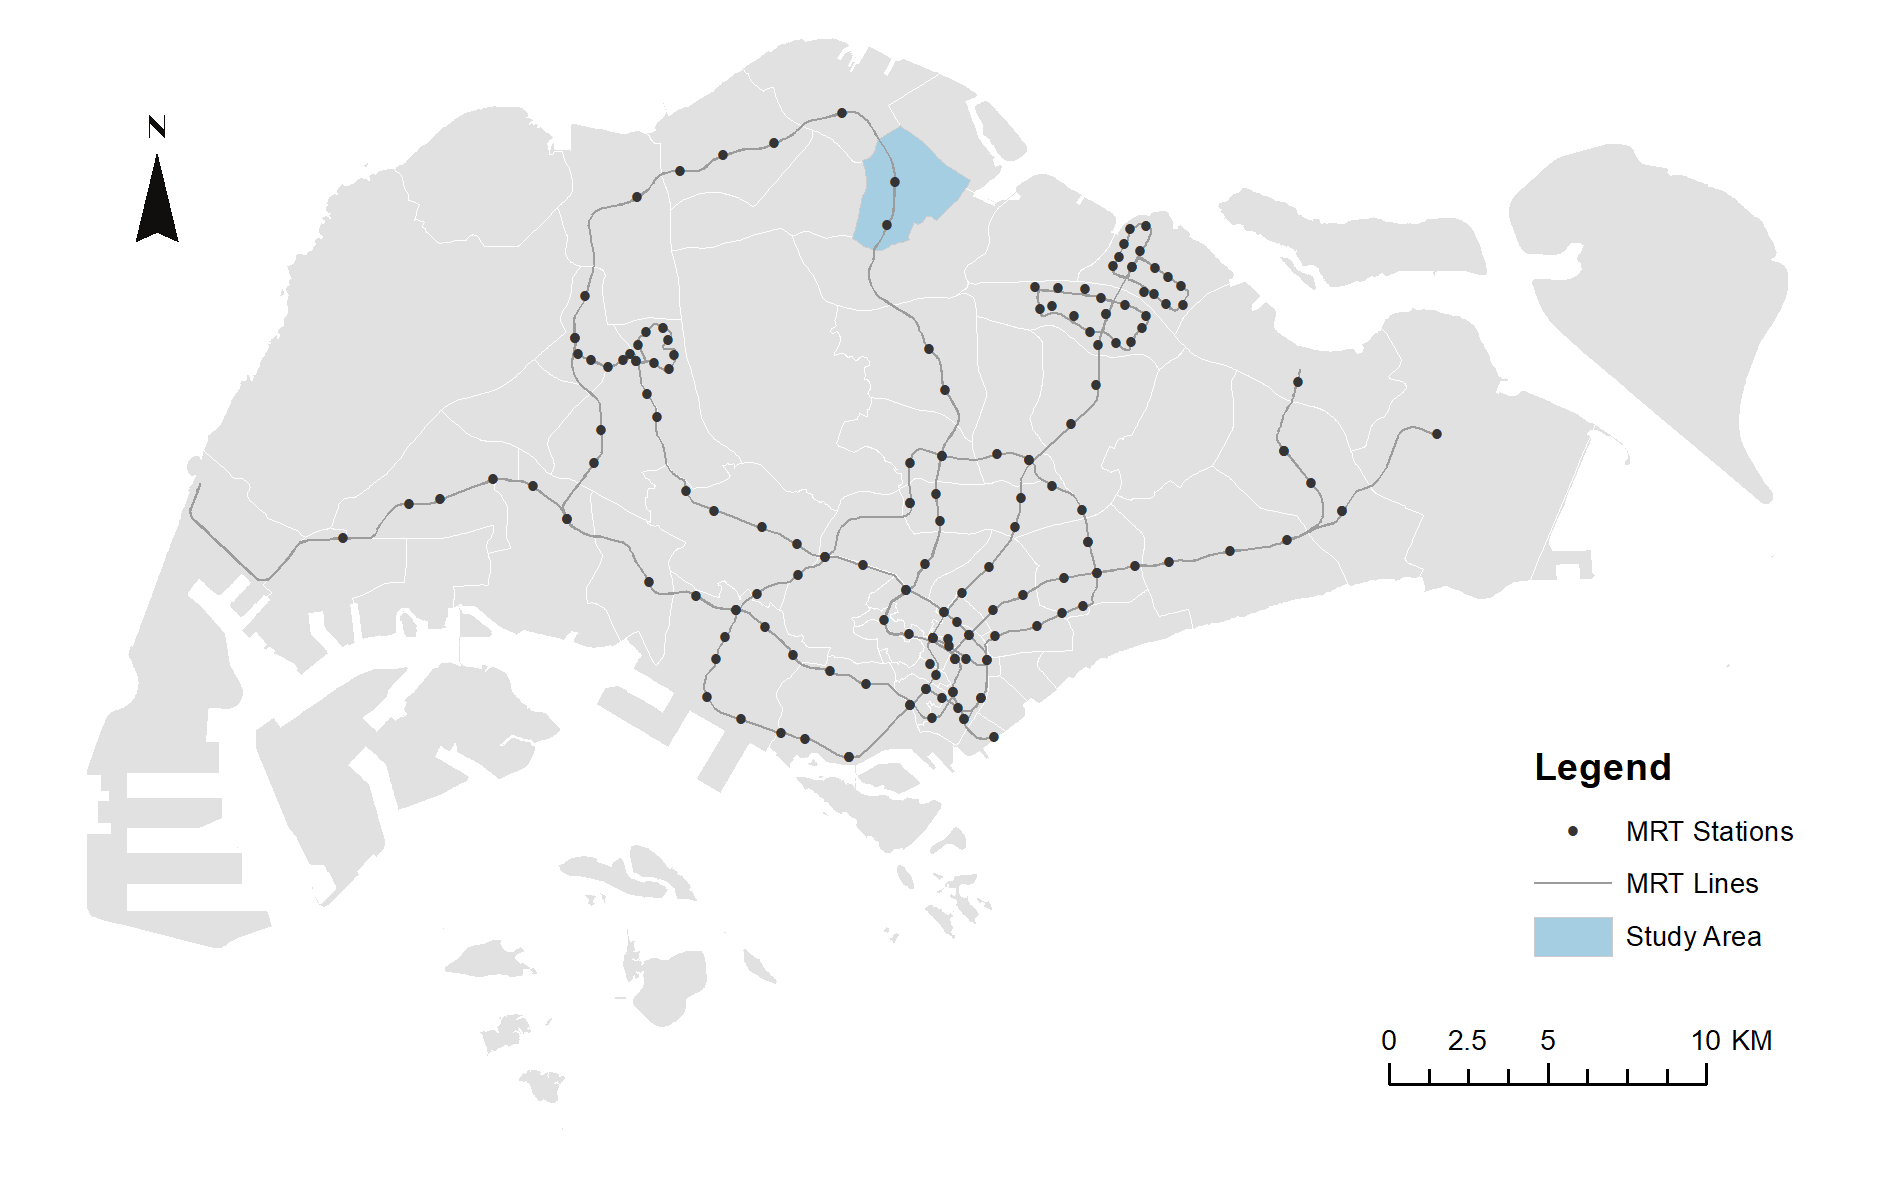
\includegraphics[width= 0.9 \textwidth]{figures_main/location_yishun.png}
	\caption{研究区域选取}
	\label{yishun}
\end{figure}

\section{实例和结果}
本节将展示如何利用构建的网络流模型解决显示问题,并对求解结果进行分析。首先,我们先在一个只有十个站点的小网络中利用模型进行求解,以方便对结果进行可视化,从而分析结果的合理性;接着,我们将实例扩大到包含更多站点,并对卡车和单车数量,调度成本,价格进行敏感性分析,这些分析将有助于我们建立对这些因素可能对收益造成的影响的更清晰认识。在敏感性分析中利用到的所有参数的所有值如表\ref{sens_case}所示。

\vspace{3mm}    %空一行
\begin{table}[H]
	\centering	
	\caption{敏感性分析参数设置}
	\label{sens_case}
	\renewcommand\arraystretch{1.5}	%行间距放大为1.5倍
	\begin
	{tabular}{p{20mm}<{\centering} p{20mm}<{\centering}}
		\toprule[2pt]
		参数 & 值 \\
		\midrule[1pt]
		调度卡车数量       & 0,1,2,3,4,5        \\
		单车数量        & 225,488,602,899     \\
		燃油成本(S\$)            & 0.4,0.6,0.8,1      \\
		定价(S\$)           & 1,1.5,2,2.5,3     \\
		\bottomrule[2pt]
	\end{tabular}
\end{table}
\vspace{3mm}

在进行敏感性分析的过程中,只改变一个参数的值,保持其它所有参数的值为默认值。卡车数量、单车数量、成本和定价的默认值分别为2,899,0.5,1。其它未提及的参数值设置均与第一步中包含十个站点的实例中相同。
我们挑选了工作日早高峰七点至十点的数据进行处理。假设在这个时间段内的任何时间切片中都可以进行调度。时间以五分钟进行切片,每个站点的单车需求也以5分钟为时间段进行计数。虽然由于未被满足的需求的存在,从单车使用数据中得到的单车需求量并不严格等于真实需求,但是由于义顺区内的单车存在过饱和,需求大于供给的情况可以忽略不计,所以在输入时仍将从数据中统计得到的使用量视为需求量。最后,将三个小时内总需求小于十的站点剔除,以减少随机需求的影响。

消费者骑行带来的收益是骑行时间的函数,这个函数中的单位价格是从新加坡目前真实的骑行定价中得到的。站点间的距离是根据站点的路网距离计算出来的。单车调度成本与每辆单车的调度都有关,具体包括单车调度过程中的磨损以及调度此辆单车需要耗费的劳动力。卡车调度成本主要指卡车油耗成本。我们还从义顺的数据中得到卡车的初始分布作为模型的初始输入。

\section{基本实例:调度行为分析}
本节将利用时空调度图将利用模型计算得到的调度计划进行可视化。基本实例中使用的参数值如下:
\begin{enumerate}
	\item 收益为S\$1每15分钟,不满15分钟按15分钟计。
	\item 卡车调度成本为S\$0.4/km。
	\item 单车调度成本为S\$0.5每辆每次
	\item 每辆卡车的容量为20
	\item 系统中调度卡车数量为3
	\item 每辆卡车的购买成本均摊到每天为S\$70(依据卡车的平均使用年限计算)
\end{enumerate}
在基本实例中,为了防止问题过于复杂难以可视化,从义顺挑选十个站点、设置调度卡车数量为三辆进行计算。这十个站点分布在义顺的两个地铁站、工业园区和社区中心附近,这些区域都是有较高共享单车需求的区域(见图\ref{selected10}),图中各自颜色的深浅代表每个站点使用的频繁程度。其中,义顺工业园和社区中心是义顺区的两个重要人口聚集地。

\begin{figure}[H]
    \centering
    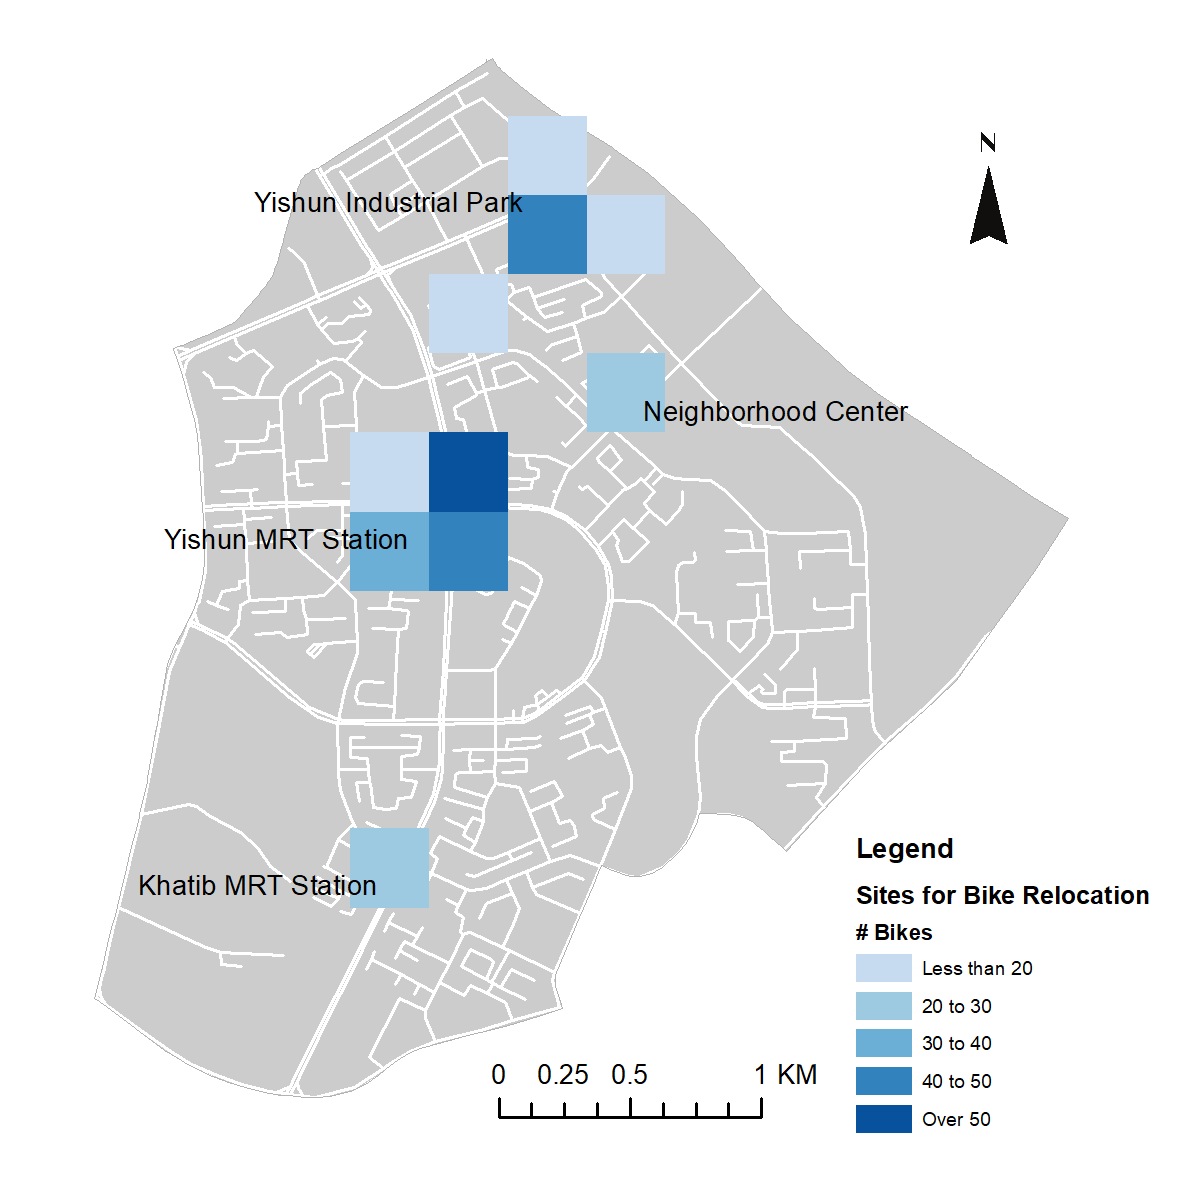
\includegraphics[width=0.5 \textwidth]{figures_main/selected_nodes10.png}
    \caption{研究区域选取}
    \label{selected10}
\end{figure}

下图\ref{visualization}中只展示了开始十二个时间切片内的计算结果。图中Yishun-1到Yishun-4表示在义顺站周围的四个站点,Industrial Park-1至Industrial Park-4表示在义顺工业中心附近的四个站点。每个圆圈的含义解释如图\ref{element_illus}所示。圆圈内的数字表示该时刻停在该站点的单车数量,圆圈上方的数组表示该时刻流入和流出该站点的单车数量。每个圆圈都含有时间和站点位置两个固定属性,在接下来的分析中,将每个圆圈称作一个“状态”。

如图\ref{visualization}所示,消费者使用单车存在明显的聚集现象,例如,在时间切片7和站点Yishun-2,被用户骑走的单车数就很大,而在其它状态下骑走的数量就相对随机。除此之外,由于社区中心离义顺工业园和义顺地铁站都在步行可达距离内,住在社区中心的人不太需要利用共享单车解决出行的第一公里和最后一公里问题,这也是在这些站点间的单车流入和流出量都很小的原因。单车调度总结起来主要发生在义顺工业园、社区中心、Khatib和Yishun两个地铁站之间。值得注意的是,调度在义顺工业园和义顺地铁站间发生的最为频繁,这是因为义顺地铁站是距离义顺工业园最近的地铁站,需要在早晚高峰通过搭乘地铁到达义顺工业园上下班的人需要频繁的来往于这两个区域之间。在在高峰,人们从义顺地铁站下地铁后需要从地铁站骑车到工业园;在晚高峰,从工业园下班的人需要骑车到义顺地铁站搭乘地铁返回。由于这两个站点间的大量共享单车需求,这两个站点间的调度也相对频繁。相比于义顺地铁站,Khatib地铁站距离社区中心和工业园都更远一些,所以从图中可以看到Khatib地铁站周围的单车使用量较少,执行的调度操作也就比较少。

对调度结果进行进一步分析可以看出,调度主要发生在早上七点至七点三十分,从义顺地铁站到义顺工业园,以及早上七点至八点,在义顺地铁站周围区域。从七点至七点半的调度高峰的出现是由于前述的糟糕分时段从地铁站至工业园的上班需求,可以理解为从七点半到八点,从义顺地铁站出发的单车需求比较大,所以需要提前准备好足够的单车使用。从七点半至八点,由于很多消费者骑车到达Yishun-1,而从Yishun-2和Yishun-4出发的需求比较大,所以需要在义顺地铁站周围的四个区域内进行单车调度以满足这些需求。

\begin{figure}[H]
    \centering
    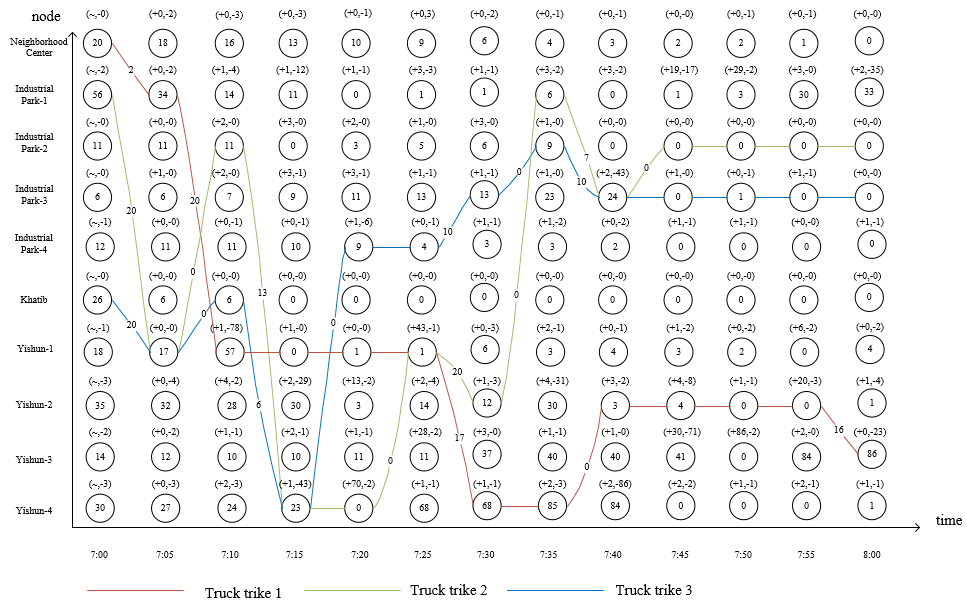
\includegraphics[width=1.0 \textwidth]{figures_main/visualiza_solution_trike.png}
    \caption{求解结果可视化}
    \label{visualization}
\end{figure}

\begin{figure}[H]
    \centering
    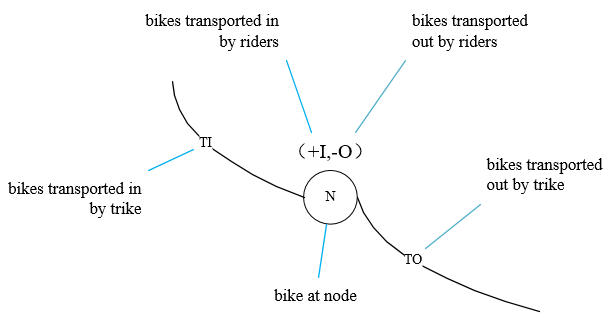
\includegraphics[width=0.5 \textwidth]{figures_main/element_illustration.png}
    \caption{元素含义解释}
    \label{element_illus}
\end{figure}

总体来说,图\ref{visualization}中展示的调度操作是符合现实情况的,并不存在异常的调度行为,如从需求量大的区域调度车辆到需求量小的区域或者在两个站点间频繁来回调度车辆。通过以上基本实例的求解和分析可以得知,通过建立的模型得到的调度计划是合理并且可执行的。
\subsection{敏感性分析}
本节主要讨论对单车和卡车数量,调度成本以及定价对收益的影响的敏感性分析结果。敏感性分析的顺序组织如下:先分析单车网络规模,即调度卡车和单车数量对收益的影响,以为如何在不同的情况下合理的决定单车和卡车数量提供一些理论支持;之后对成本和定价这两个直接影响收益的核心因素核心因素对最终收益的影响进行敏感性分析。正确理解单车数量、调度卡车数量、成本和定价对收益的影响是决定运营的共享单车网络是否能稳定维持的关键。敏感性分析中涉及到的参数值已在表\ref{studied scenarios}中给出。


\begin{table}[H]
	\centering
	\caption{研究场景}
	\label{studied scenarios}
	\renewcommand\arraystretch{1.5}
	\begin{tabular}{p{20mm}<{\centering} p{20mm}<{\centering} p{20mm}<{\centering} p{20mm}<{\centering} p{20mm}<{\centering}}
	\toprule[2pt]
     & 卡车数量 & 单车数量 & 燃油成本(S\$) & 定价(S\$) \\
	\midrule[1pt]
	\multirow{6}{*}{\begin{tabular}[c]{@{}c@{}}对卡车数量\\ 敏感性分析\end{tabular}} & 0                      & 899                   & 0.5               & 1                  \\
																							   & 1                      & 899                   & 0.5               & 1                  \\
																							   & 2                      & 899                   & 0.5               & 1                  \\
																							   & 3                      & 899                   & 0.5               & 1                  \\
																							   & 4                      & 899                   & 0.5               & 1                  \\
																							   & 5                      & 899                   & 0.5               & 1                  \\ 
																				\midrule[1pt]
	\multirow{4}{*}{\begin{tabular}[c]{@{}c@{}}对单车数量\\ 敏感性分析\end{tabular}}  & 2                      & 225                   & 0.5               & 1                  \\
																							   & 2                      & 488                   & 0.5               & 1                  \\
																							   & 2                      & 602                   & 0.5               & 1                  \\
																							   & 2                      & 899                   & 0.5               & 1                  \\
																				\midrule[1pt]
	\multirow{4}{*}{\begin{tabular}[c]{@{}c@{}}对成本\\ 敏感性分析\end{tabular}}           & 2                      & 899                   & 0.4               & 1                  \\
																							   & 2                      & 899                   & 0.6               & 1                  \\
																							   & 2                      & 899                   & 0.8               & 1                  \\
																							   & 2                      & 899                   & 1                 & 1                  \\
																				\midrule[1pt]
	\multirow{5}{*}{\begin{tabular}[c]{@{}c@{}}对定价\\ 敏感性分析\end{tabular}}          & 2                      & 899                   & 0.5               & 1                  \\
																							   & 2                      & 899                   & 0.5               & 1.5                \\
																							   & 2                      & 899                   & 0.5               & 2                  \\
																							   & 2                      & 899                   & 0.5               & 2.5                \\
																							   & 2                      & 899                   & 0.5               & 3                  \\
	\bottomrule[2pt]
	\end{tabular}
\end{table}

除了对收益进行敏感性分析,本研究同样对消费者满意度进行了敏感性分析。收益代表的是网络的短期盈利能力,想要长期的稳定占有市场,消费者满意度是不可以忽略的。消费者满意度的定义为:
\begin{center}
满意度=满足的需求数量/总需求
\end{center}
\noindent
其中,满足的需求数量是指在期望出发点找到可用单车的消费者数量。

作为基本实例的延申,在进行敏感性分析时,我们在义顺区选择了23个站点进行计算,这23个站点是所有站点中使用最为频繁的前23个站点。这些站点的位置如图\ref{selected}所示。
\begin{figure}[H]
    \centering
    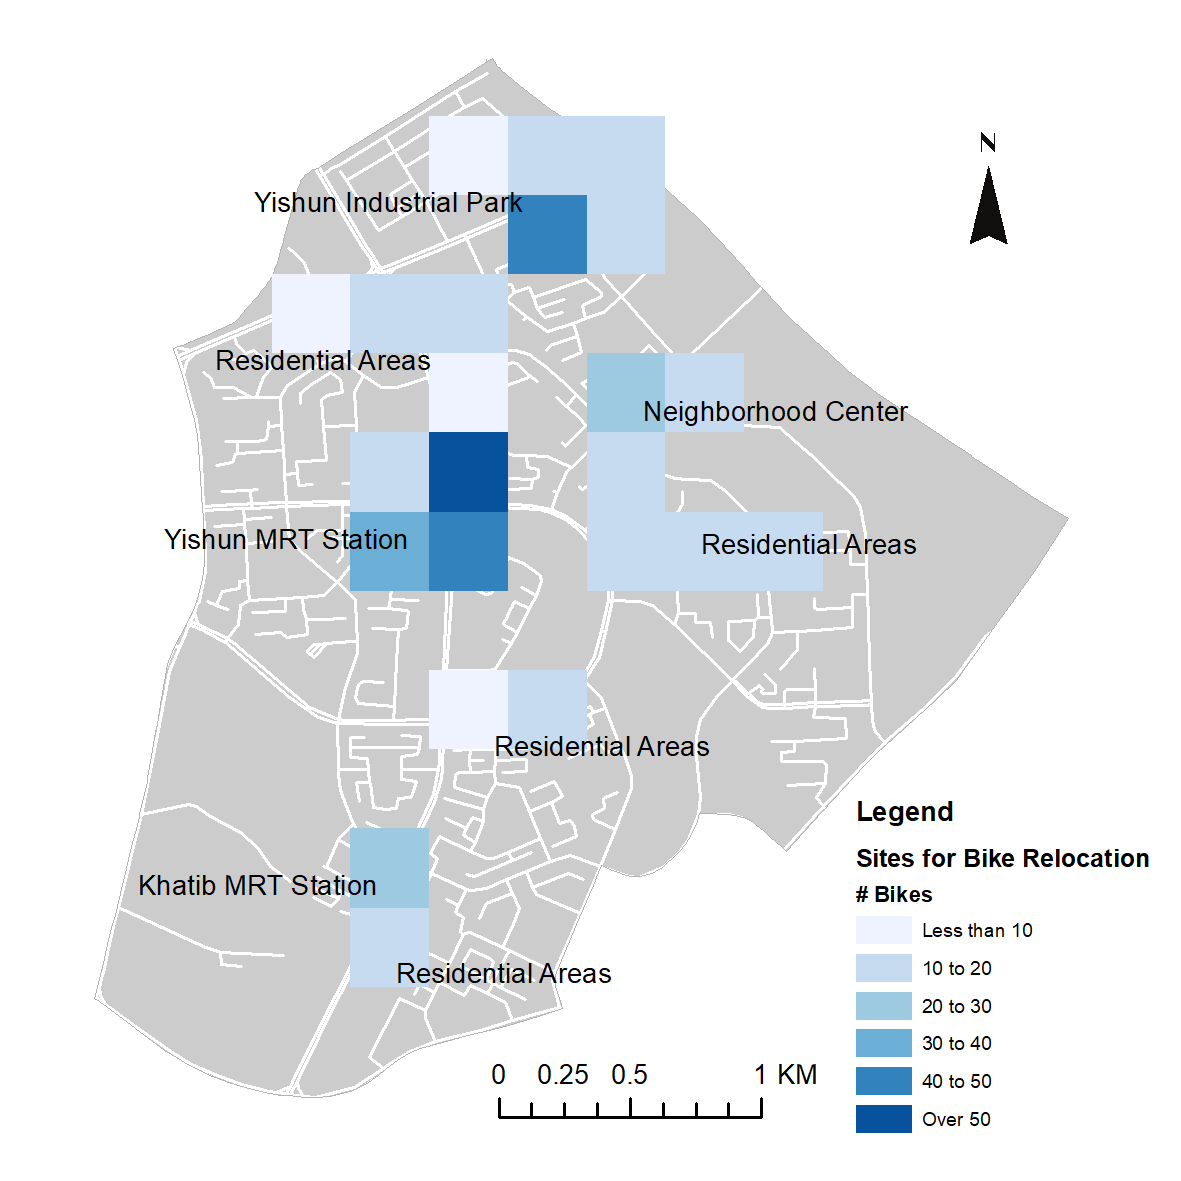
\includegraphics[width= 0.5\textwidth]{figures_main/selected_nodes.png}
    \caption{新研究区域选取}
    \label{selected}
\end{figure}
\subsection{网络规模敏感性分析}
共享单车网络的管理需求可以分为以下两两个场景:
\begin{enumerate}
	\item 在固定网络规模(单车数量)的情况下,共享单车网络运营商期望通过尽可能少的调度实现利润最大化。
	\item 共享单车运营商希望在一片新的区域建立共享单车网络,期望尽可能少的投放单车实现利润最大化。
\end{enumerate}

以下在这两个场景中进行敏感性分析。

在第一个场景下,我们进行在固定单车数量时,卡车数量对于利润的敏感性分析。利用义顺的实际数据计算得到的结果如图\ref{sens_trike}所示。图中每个坐标点代表一个实例,所有的实例都是在三十分钟的计算时间限制下计算得到的。如图\ref{sens_trike_no}所示,当不考虑购买卡车的成本时,收益随着卡车数量增加持续上升,但上升速度逐渐减慢最终趋于稳定;在图\ref{sens_trike_with}中,收益和乘客满意度先随卡车数量的增加而上升,当卡车数量为2时达到峰值,之后收益随卡车数量的上升而下降。图\ref{sens_trike_no}中的峰值点之所以存在是因为卡车数量增多带来的调度能力增加可以部分缓解某些站点单车数量不足的情况,使得网络能够满足更高的单车需求量,但同时,购买更多的卡车意味着更高的运营成本,所以一味地通过购买卡车来提高网络运载能力以提高收益是不合理的。卡车的数量需要综合网络的现实情况决定才可能达到图中的峰值。
\begin{figure}[H]
	\centering
	\subfloat[不考虑卡车购买成本]{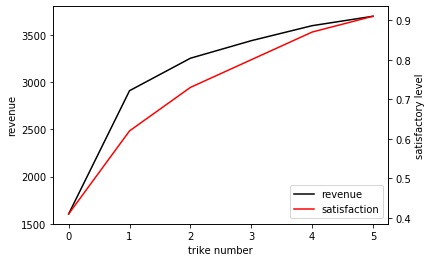
\includegraphics[width=0.5\textwidth]{figures_main/sens_trike_notrikecost.png}\label{sens_trike_no}}
	\hfil
	\subfloat[考虑卡车购买成本]{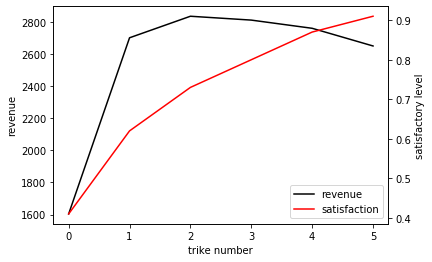
\includegraphics[width=0.5\textwidth]{figures_main/sens_trike_70.png}\label{sens_trike_with}}
	\hfil
	\caption{卡车数量敏感性分析}
	\label{sens_trike}
\end{figure}

为了进一步分析在不同系统规模,即单车数量的情况下卡车数量对收益的影响,我们分别在单车数量为899(实际规模)、499时计算卡车数不同时的系统收益。减小单车数量通过将每个站点的初始共享单车量同比例缩小达到。计算结果如图\ref{trike_compare}所示。从图中可以看出,有448辆共享单车,两辆调度卡车的共享单车系统的盈利高于有899辆单车,无调度用车的系统,这正说明在合适选择卡车数量的情况下,拥有更少共享单车的系统的盈利能力可以超过有更多共享单车的系统。所以,不需要为了提高收益一味的增加共享单车投放量,调度是除了增加单车投放量之外的一种有效提升系统满足需求能力的手段。

\begin{figure}[H]
    \centering
    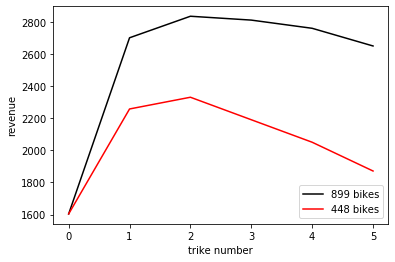
\includegraphics[width=0.5 \textwidth]{figures_main/sens_trike_compare.png}
    \caption{不同单车数量分析}
    \label{trike_compare}
\end{figure}

在第二个场景中,我们进行在调度卡车数量一定时,单车数量对于收益的敏感性分析。将卡车数量设为2,敏感性分析得到的结果如图\ref{sens_bike}所示。图中显示,消费者满意度随单车数量的上升持续上升。这一点很好理解,因为从消费者的角度看,更多的单车意味着他们有更高的机率能在自己的期望出发点找到可用的单车。另外,尽管从图中看来系统的收益也随单车数量的增多而上升,但这并不意味着更多的单车能够带来更多的利润,这是因为我们在场景二下进行对单车数量的敏感性分析,这意味着我们的假设是这是一个新的或者需要改变规模的系统,所以此时单车购买的成本应计入总成本中,而前述模型的目标函数并没有加上这一部分成本。由于单车数是我们在优化前就给定的,所以这部分成本为固定值,可以直接在求解结果中减去求出实际收益。假设一辆共享单车的使用寿命为一年,那么购买一辆单车的花销可以均摊到每天,设为S\$1.5。减去这部分成本后的结果如表\ref{sens_profit}所示。从表中可以看出,单车数量和系统收益间没有明显的单一正相关或者负相关关系。事实上,最终的收益和很多因素都有关,比如单车的使用寿命、价格以及消费者对待单车的方式。由于这些因素在不同地区的差别可以很大,难以给出比较具有普适性的参数值,所以在决定单车数量时,应先全面考虑这些因素,以及结合单车系统所处的不同状态,确定合适参数值以及期望达到的目标后再进行计算。单车系统所处的状态对于期望达到的目标的影响是指:对于一个新的共享单车系统,消费者满意度通常是决定这个新的运营商是否能取得消费者信赖的关键指标;但当共享单车系统的运营已经进入了一个比较稳定的阶段,已经在消费者心中建立了信任体系后,系统的盈利水平会是维持运营的一个更重要因素。
\begin{figure}[H]
    \centering
    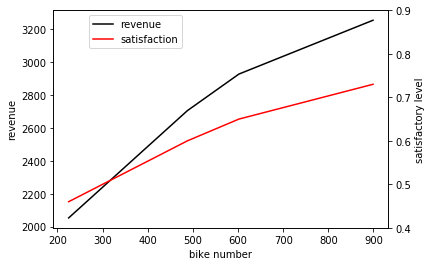
\includegraphics[width=0.5 \textwidth]{figures_main/sensitivity_bike.png}
    \caption{单车数量敏感性分析}
    \label{sens_bike}
\end{figure}

\begin{table}[H]
    \centering
    \caption{纯利润对单车数量的敏感性}
    \label{sens_profit}
    \begin{tabular}{c|c|c}
    \hline
    \textbf{Number of bikes} &\textbf{Number of trikes} &\textbf{Profit}\\
    \hline
    899 &2 &1905\\
    602 &2 &2024\\
    488 &2 &2033\\
    225 &2 &1715\\
    \hline
    \end{tabular}
\end{table}

\subsection{调度成本敏感性分析}
在本节中,我们讨论调度成本对于模型结果的影响。这里的成本指的是燃油成本,因为这个成本会随着交通状况变化,而单车损耗和搬运的成本相对固定。本节中的所有计算实例都假设系统有899辆单车和2辆调度卡车。结果如图\ref{sens_cost}所示。有结果计算可得。当成本翻倍时,系统收益只下降了2\%,而消费者满意度基本维持不变。这是由于一辆车的燃油成本是需要均摊到运送的每辆单车上的,例如,如果一辆卡车上运载了20辆单车,那么每辆单车带来的燃油成本就是总成本除以20,所以调度成本的增加对收益的影响没有前面讨论的系统规模对收益的影响那么显著。
\begin{figure}[H]
    \centering
    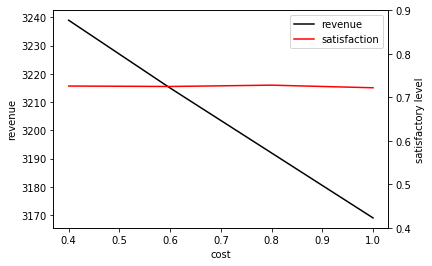
\includegraphics[width=0.5 \textwidth]{figures_main/sensitivity_cost.png}
    \caption{成本敏感性分析}
    \label{sens_cost}
\end{figure}

\subsection{定价敏感性分析}
由于定价是决定共享单车系统是否能长期稳定运营的一个核心因素,所以在本节中,我们讨论定价对收益的影响规律。和前面几节一样,在改变单车使用价格时,我们假设这个系统中拥有899辆单车和2辆调度卡车。

在前面进行的敏感性分析中,由于定价总是固定的,所以我们仍认为消费者满意度是满足的需求与总需求的比值,且乘客对价格不敏感。但在现实世界中,消费者通常情况下都是对价格敏感的,价格的上升会使需求量下降。所以在本节中改变定价时,我们利用Kaviti等的文章中阐述的需求与定价的关系\cite{kaviti2019assessing},在价格改变时同样改变输入的需求量。图\ref{sens_price}展示了得到的结果。由图中可知,定价与系统收益的关系并不是单一的正相关或负相关关系,这是由于在价格变化时,需求量也会相应变化。但是,消费者满意度会随着定价持续上身,这是因为价格上升时需求量下降,在系统单车数量不变的情况下,这意味着每个有需求的用户在期望出发点找到可用车辆额概率上升。和4.4.1相同,在不同阶段,对收益和乘客满意度这两者的考虑需要分别权衡,得到合适的定价策略。
\begin{figure}[H]
    \centering
    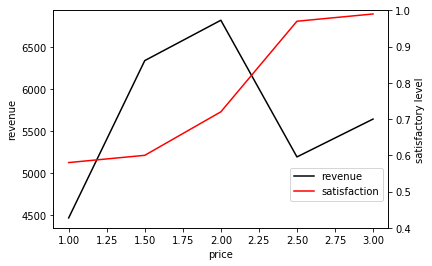
\includegraphics[width=0.5 \textwidth]{figures_main/sensitivity_price.png}
    \caption{定价敏感性分析}
    \label{sens_price}
\end{figure}

\subsection{模型延申:增加站点容量的限制的共享单车系统}
正如开头所说,有桩共享单车的历史比无桩共享单车长很多,并且在现有研究中,有桩共享单车常常被当作共享单车系统的典型运营模式进行研究。为了使我们的模型适用于有桩共享单车系统,只需要在原来的模型基础上增加一个每个站点的容量约束即可。以往对有桩共享单车系统的研究中,大多数都将调度问题看作一个车辆路径规划问题,强调如何规划最优的调度路线以消除期望单车分布和实际单车分布间的差别\cite{chemla2013bike,liu2016rebalancing,pfrommer2014dynamic},而本研究从不同的角度分析调度这个问题。在我们的模型中,我们并不关注调度的具体路线,而关注整个系统的调度计划。除此之外,我们的模型始终关注的是系统收益,而之前的研究主要关注如何利用调度提升用户服务,也就是说,提高消费者在期望始发地找到可用车辆,在期望目的地有空余停车桩的概率。

将以下约束加入模型中,得到适合有桩共享单车网络的模型:
\begin{align}
    {b_{i}^{t}}{\leq cap, \;  \forall i\in N, t \in T}
\end{align}
\noindent
$cap$代表每个站点给定的桩的数量。

为了比较有桩和无桩两种共享单车系统在利用此模型求解时的结果差异,我们使用与基础实例中相同的参数值和初始单车分布、需求值求解有桩共享单车和无桩共享单车网络的模型实例并进行比较。由于从新加坡的真实数据中得到的单车分布具有高空间不平衡的特征,比如在一些点存放的共享单车数量超过另一些点的十倍,在有桩共享单车实例中,我们需要设置站点容量为很高的值以保证从数据中获得的单车初始分布满足容量限制约束。然而,设置站点容量值过高会使得站点容量的约束成为多余的约束,因为在之后的求解中容量可能总大于需要停放的单车数量。为了解决这个问题,我们把每个站点的初始单车分布等比例缩放至均小于30,再将站点容量从30提高到70观察收益变化。在所有实例中,选择系统中的十个站点,并设置调度卡车数量为三辆,其它参数和基础实例中设置的相同。求解结果如图\ref{revenue_cap}所示。
\begin{figure}[H]
    \centering
    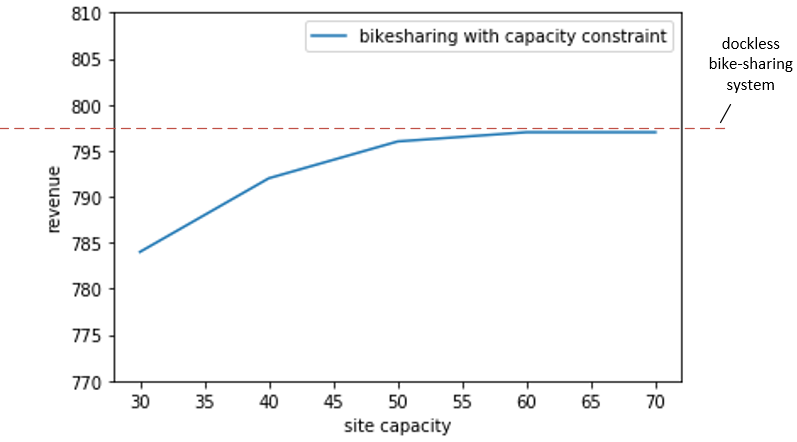
\includegraphics[width=0.5\textwidth]{figures_main/revenue_change_with_capacity.png}
    \caption{收益随站点容量变化}
    \label{revenue_cap}
\end{figure}

从上图中可以看出,随着站点容量的上升,有桩共享单车系统的收益也上升。当站点容量达到60时,有桩共享单车系统与相同规模、属性的无桩共享单车系统收益相等。这个结果证明通过在每个站点设置合适数量的停车桩,有桩共享单车系统的表现就能和无桩共享单车系统相同,并且兼有有桩和无桩共享单车系统的优势:(1)此系统能像无桩共享单车系统一样满足任何的归还车辆需求(2)此系统具有有桩共享单车系统的易于管理的优点。停车桩的建设也是成本的一部分,为了进一步在有桩共享单车系统中降低成本,可以在模型求解过程中,对每个站点的停车桩数量根据大致需求设置不同的值。这样一来,这个增加站点停车数量约束限制的模型就可以有效的为有桩共享单车网络的设计提供依据。
\clearpage
\chapter{总结与讨论}
在本研究中,我们定义了一个混合整数优化问题和一个网络流模型用以解决共享单车网络的日常调度计划设计问题。之后,我们利用了新加坡义顺区的实际共享单车使用数据,将其处理为模型需要的输入,对模型进行了应用实例的测试。在证明了模型的有效性的基础上,我们又利用此模型对网络规模、成本和定价对网络收益的影响进行了敏感性分析,在分析的过程中除了研究收益之外,我们对这些因素造成的消费者满意程度的变化也进行了讨论,因为消费者满意程度是衡量网络运营质量的关键指标。之后作为模型的延申,我们在原模型的基础上加入了站点容量约束,用于解决无桩共享单车的调度问题。最后,我们利用这个延申模型分析了有桩和无桩共享单车间的关系。

对于一个已知单车数量的共享单车系统,卡车数量对系统收益的影响可以直接利用本文中构建的模型进行分析,并帮助运营商管理调度。然而,当需要为一个新的共享单车系统决定合适的共享单车投放量时时,问题就会变得更加复杂。正如上一节所讨论的,对于一个新的或者需要改变规模的共享单车系统,可以通过两种途径尽可能提高系统收益。第一种途径是在系统中投放更多单车,第二种是在系统中投放更多卡车用于调度。由于无桩共享单车还处在发展阶段,为了提高市场占有率,很多运营商为了提高自己的市场竞争力一味地加大共享单车投放量,这是十分没有必要的。这种过度投放也使得一些共享单车项目最终走向破产,因为过多单车不但会提高购买成本,也会大大提高后期的运营成本。除了对受益的影响,共享单车的过度投放也会造成公共空间的浪费,这对城市管理者来说也是一个挑战。尽管共享单车的使用能够有效减少碳排放,其对空间资源的占用还是会造成环境问题。如果碳排放的减少需要以空间资源的浪费为代价,那么共享单车的使用是否是一个环保的出行方式就更有待商榷。

延申模型展示了一个很好理解的规律:通过增大站点的停车桩数量,一个有桩共享单车网络可以转变为无桩共享单车网络。但是,每个站点具体设置多少停车桩合理还需要进一步研究计算。

通过本研究对共享单车网络运营规律和管理的分析和理解,最后我们可以给出如下对网络运营和管理上的建议:
\begin{enumerate}
	\item  改变共享单车网络的管理模式。在本研究中,我们并没有在所有的计算实例中考虑共享单车的购买成本,因为我们主要在固定网络规模的共享单车系统中考虑各个因素对收益的影响,所以可以看作共享单车购买这一步已经完成。在未考虑单车购买成本的情况下,共享单车项目看起来是很有盈利空间的。但是在现实世界中,共享单车项目走向破产的情况屡见不鲜,这是因为在实际运营中,车辆的损坏和丢失无法避免,所以在单车购买上通常需要持续投入。由于单车购买的投入太大,运营商难以长期维持系统运营,导致在现实中一些共享单车系统缺乏盈利能力。我们建议,缓解这个问题的途径之一可以考虑改变共享单车系统目前的运营结构。除了运营商自生之外,应让政府部门也参与到决定网络中投放的共享单车数量中,并且政府部门对单车运营商进行单车购买的补贴,单车数量由系统的盈利能力和将占用的公共空间共同决定。在限制单车数量的调节下,运营商可以自主指定调度计划管理整个网络。网络最终的收益有运营商和政府共同享有。这种运营模式有诸多好处,例如,城市管理者可以通过设置单车数量限制减少单车将占用的公共空间资源,协调城市管理;运营商可以降低系统构建和运营成本,获得更多利润。这些综合起来将为城市居民提供高质量的共享单车服务,不仅方便出现,同样也环境友好。
	\item  共享单车数量应有限制。从延申模型中得到的结果证明合理的设置每个站点停靠的单车数量并不会大大降低系统的盈利能力。共享单车过饱和不仅会提高系统运营成本,也会造成空间资源浪费,使得城市管理更加困难。所以,城市管理者可以设置共享单车的数量限制,设置数量限制并不会显著降低运营商的盈利或者降低服务质量。
\end{enumerate}
随着共享单车系统在越来越多的城市落地,调度问题的场景也越来越多样、越来越复杂。未来的研究还需要继续关注这些不同的调度场景下的调度问题。以下提出一些研究点作为未来的研究讨论的方向的参考。在本研究中,为了简化模型构建,我们做了很多假设和简化。事实上,为了使模型贴合实际,更多更符合现实的因素应该被考虑,比如消费者在站点等待可用单车或者移动到附近站点寻找可用单车,这将会影响消费者满意率的计算。消费者满意率同样也需要更精细的定义。至于调度手段,除了运营商通过配置卡车进行统一调度,使用骑行激励,即利用骑车补贴鼓励消费者改变期望目的地实现调度的方式也是一种有效的调度策略。除以上这些之外,进一步的研究也可以着眼于寻找更高效的模型求解算法,因为随着问题规模的扩大,求解难度也会大大上升。无桩共享单车的模型规模由于其停车点的随机性要远大于有桩共享单车系统。最后,在本研究所讨论的网络流量模型中,每辆调度卡车的调度路线是被模糊化处理的,如果想要制订更精细的调度策略,未来的研究可以考虑把车辆路径规划问题整合到目前的模型中。
\clearpage
\begin{comment}
\vspace{3mm}    %空一行
\begin{table}[H]
	\centering	
	\renewcommand\arraystretch{1.5}	%行间距放大为1.5倍
	\begin
	{tabular}{p{17mm}<{\centering} p{10mm}<{\centering} p{10mm}<{\centering} p{25mm}<{\centering} p{20mm}<{\centering} p{10mm}<{\centering} p{10mm}<{\centering} p{20mm}<{\centering}}
		\toprule[2pt]
		Message & ID & CycleTime & Signal & ValueType & length & Factor & C Type \\
		\midrule[1pt]
		SetPoints & 0x02 & 10 & Reserved & Unsigned & 6 & 1 &  \\
		SetPoints &  & 10 & Enable & unsigned & 1 & 1 & unsigned char \\
		SetPoints &  & 10 & ErrorReset & unsigned & 1 & 1 & unsigned char \\
		SetPoints &  & 10 & TargetTorque & signed & 16 & 0.0098 & short \\
		SetPoints &  & 10 & TorqueLimitP & signed & 16 & 0.0098 & short \\
		SetPoints &  & 10 & TorqueLimitN & signed & 16 & 0.0098 & short \\
		SetPoints &  & 10 & Reserved & Unsigned & 8 & 1 &  \\
		\midrule[1pt]
		Message &  & CycleTime & Signal & ValueType & length &  &  \\
		SetPoints & 0x00 & 10 & Reserved & Unsigned & 6 & 1 &  \\
		ActualValues1 &  & 5 & Enabled & unsigned & 1 & 1 & unsigned char \\
		ActualValues1 &  & 5 & Error & unsigned & 1 & 1 & unsigned char \\
		ActualValues1 &  & 5 & DCVoltage & unsigned & 16 & 1 & unsigned short \\
		ActualValues1 &  & 5 & ActualTorque & signed & 16 & 0.0098 & short \\
		ActualValues1 &  & 5 & ActualVelocity & signed & 16 & 1 & short \\
		ActualValues1 &  & 5 & Diagnostic & unsigned & 8 & 1 & unsigned char \\
		% \midrule[1pt]
		ActualValues2 & 0x04 & 500 & TempMotor & unsigned & 16 & 0.1 & unsigned short \\
		ActualValues2 &  & 500 & TempInverter & unsigned & 16 & 0.1 & unsigned short \\
		ActualValues2 &  & 500 & TempIGBT & unsigned & 16 & 0.1 & unsigned short \\
		ActualValues2 &  & 500 & Reserved & Unsigned & 16 & 1 &  \\

		\bottomrule[2pt]
	\end{tabular}
	\caption{message表格}
\end{table}
\vspace{3mm}
\end{comment}

\addcontentsline{toc}{chapter}{参考文献}
%\chapter*{参考文献}
{
	\hyphenpenalty=1000 %断词阈值,值越大越不容易出现断词
	\tolerance=500 %丑度,10000为最大无溢出盒子
	\hbadness=100 %如果丑度超过hbadness这一阀值,那么就会发出警告
	\printbibliography[]
}
\clearpage
% \addcontentsline{toc}{chapter}{本科就读期间取得的学术成果}
% \chapter*{本科就读期间取得的学术成果}
% \begin{enumerate}
% 	\item 1
% 	\item 2
% 	\item 3
% 	\item 4
% \end{enumerate}
% \clearpage
\addcontentsline{toc}{chapter}{致~谢}
\chapter*{致~谢}
我衷心感谢\textsc{TongjiThesis}对我的论文的帮助,帮助我节约了不少时间。非常感谢!


\end{document}
